\chapter{彭庆福餐厅点单系统的详细设计与实现}
本章主要介绍了彭庆福餐厅点单系统的各个功能模块,分析了模块之间的依赖关系,具体描述了各模块的详细设计与实现细节。
\section{模块设计}
\begin{figure}[htbp!]
    \centering
    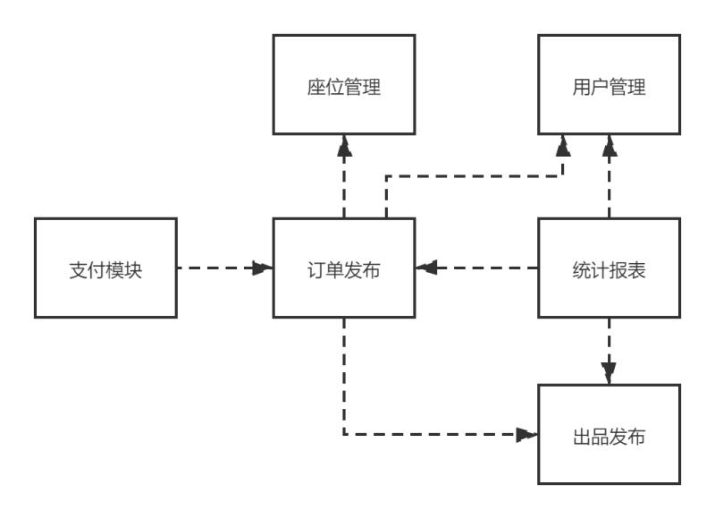
\includegraphics[width=4in]{FIGs/chapter4/model.pdf}
    \caption{系统模块结构图}\label{fig_model}
\end{figure}

彭庆福餐厅点单系统划分为六个模块,分别是订单发布模块、支付模块、用户管理模块、统计报表模块、座位管理模块和出品发布模块。模块之间的相互依赖如图~\ref{fig_model}所示,支付模块依赖订单发布模块,订单发布模块依赖座位管理模块、出品发布模块以及用户管理模块,统计报表模块依赖订单发布模块、出品发布模块以及用户管理模块~\cite{sjb2019}。以下分别对不同模块进行介绍:

\begin{enumerate}
    \item 订单发布模块是整个系统中最主要的模块,它负责处理与顾客下单后的订单有关的操作,订单发布主要包括用户信息、座位信息以及菜品信息,对外提供订单列表、订单详情相关服务的接口。
    \item 支付模块依赖于订单发布,主要负责处理顾客支付时的支付安全和第三方支付,包括微信支付、支付宝支付等。
    \item 用户管理模块主要负责处理与用户各种信息有关的操作,系统一共有两大类用户,顾客和商家,用户管理模块主要对外提供顾客信息服务、角色服务、商家信息服务等接口。
    \item 统计报表模块主要负责收集、整合各个报表信息,主要对外提供不同时间段的收入报表、菜品进销存报表、下载报表的接口。
    \item 座位管理模块主要负责处理座位有关的操作,主要对外提供座位信息、座位二维码、座位状态等接口~\cite{dj2019}。
    \item 出品发布模块主要负责每日出品计划、菜品计划,用于每天的营业时间、菜品管理等问题的处理,主要对外提供商家营业信息、出品计划、菜品信息等接口。
\end{enumerate}

下面对这六个模块分别进行介绍。\\

\section{订单发布模块}
\subsection{订单发布模块介绍}
订单发布模块是整个系统中最主要的模块,它负责处理与顾客下单有关的操作,顾客可以选菜下单,创建订单、查询订单、取消订单,商家可以查看所有顾客订单以及对具体订单进行操作。订单发布主要包括用户信息、座位信息以及菜品信息,支付模块以及统计报表模块都需要依赖它。

订单发布模块需要多类状态综合判断,通过顾客状态(已到店、已离店)、商家处理订单状态、以及支付状态(待支付、已支付、支付失败)来决定订单状态(已提交待确认、进行中、已结束未评价、取消、已取消未评价、已结束已评价)。

订单发布模块会展示三种类型的订单详情,一种是到店订单类型,一种是预约订单类型,还有一种是外卖订单类型,多位顾客同时在线下单,后台会根据具体时间对订单排序生成特定订单编号~\cite{hsp2017}。顾客每次下单都会根据不同类型生成相应订单,商家可以在订单发布里查看到所有的订单列表,点击具体订单可以查看订单详情,进行相应的操作,比如修改顾客用餐人数、确认顾客离店、打印菜单、结账等。\\

\subsection{订单发布模块详细设计}
订单发布模块包括顾客点单部分和商家管理订单部分,其中还涉及到了生产计划服务、用户服务、订单条目服务等。如图~\ref{fig_order}所示是订单发布模块的类图,主要实现了与订单相关的内容,需要依赖发布服务、生产计划服务、用户服务、订单条目等内容。

\begin{figure}[htbp!]
    \centering
    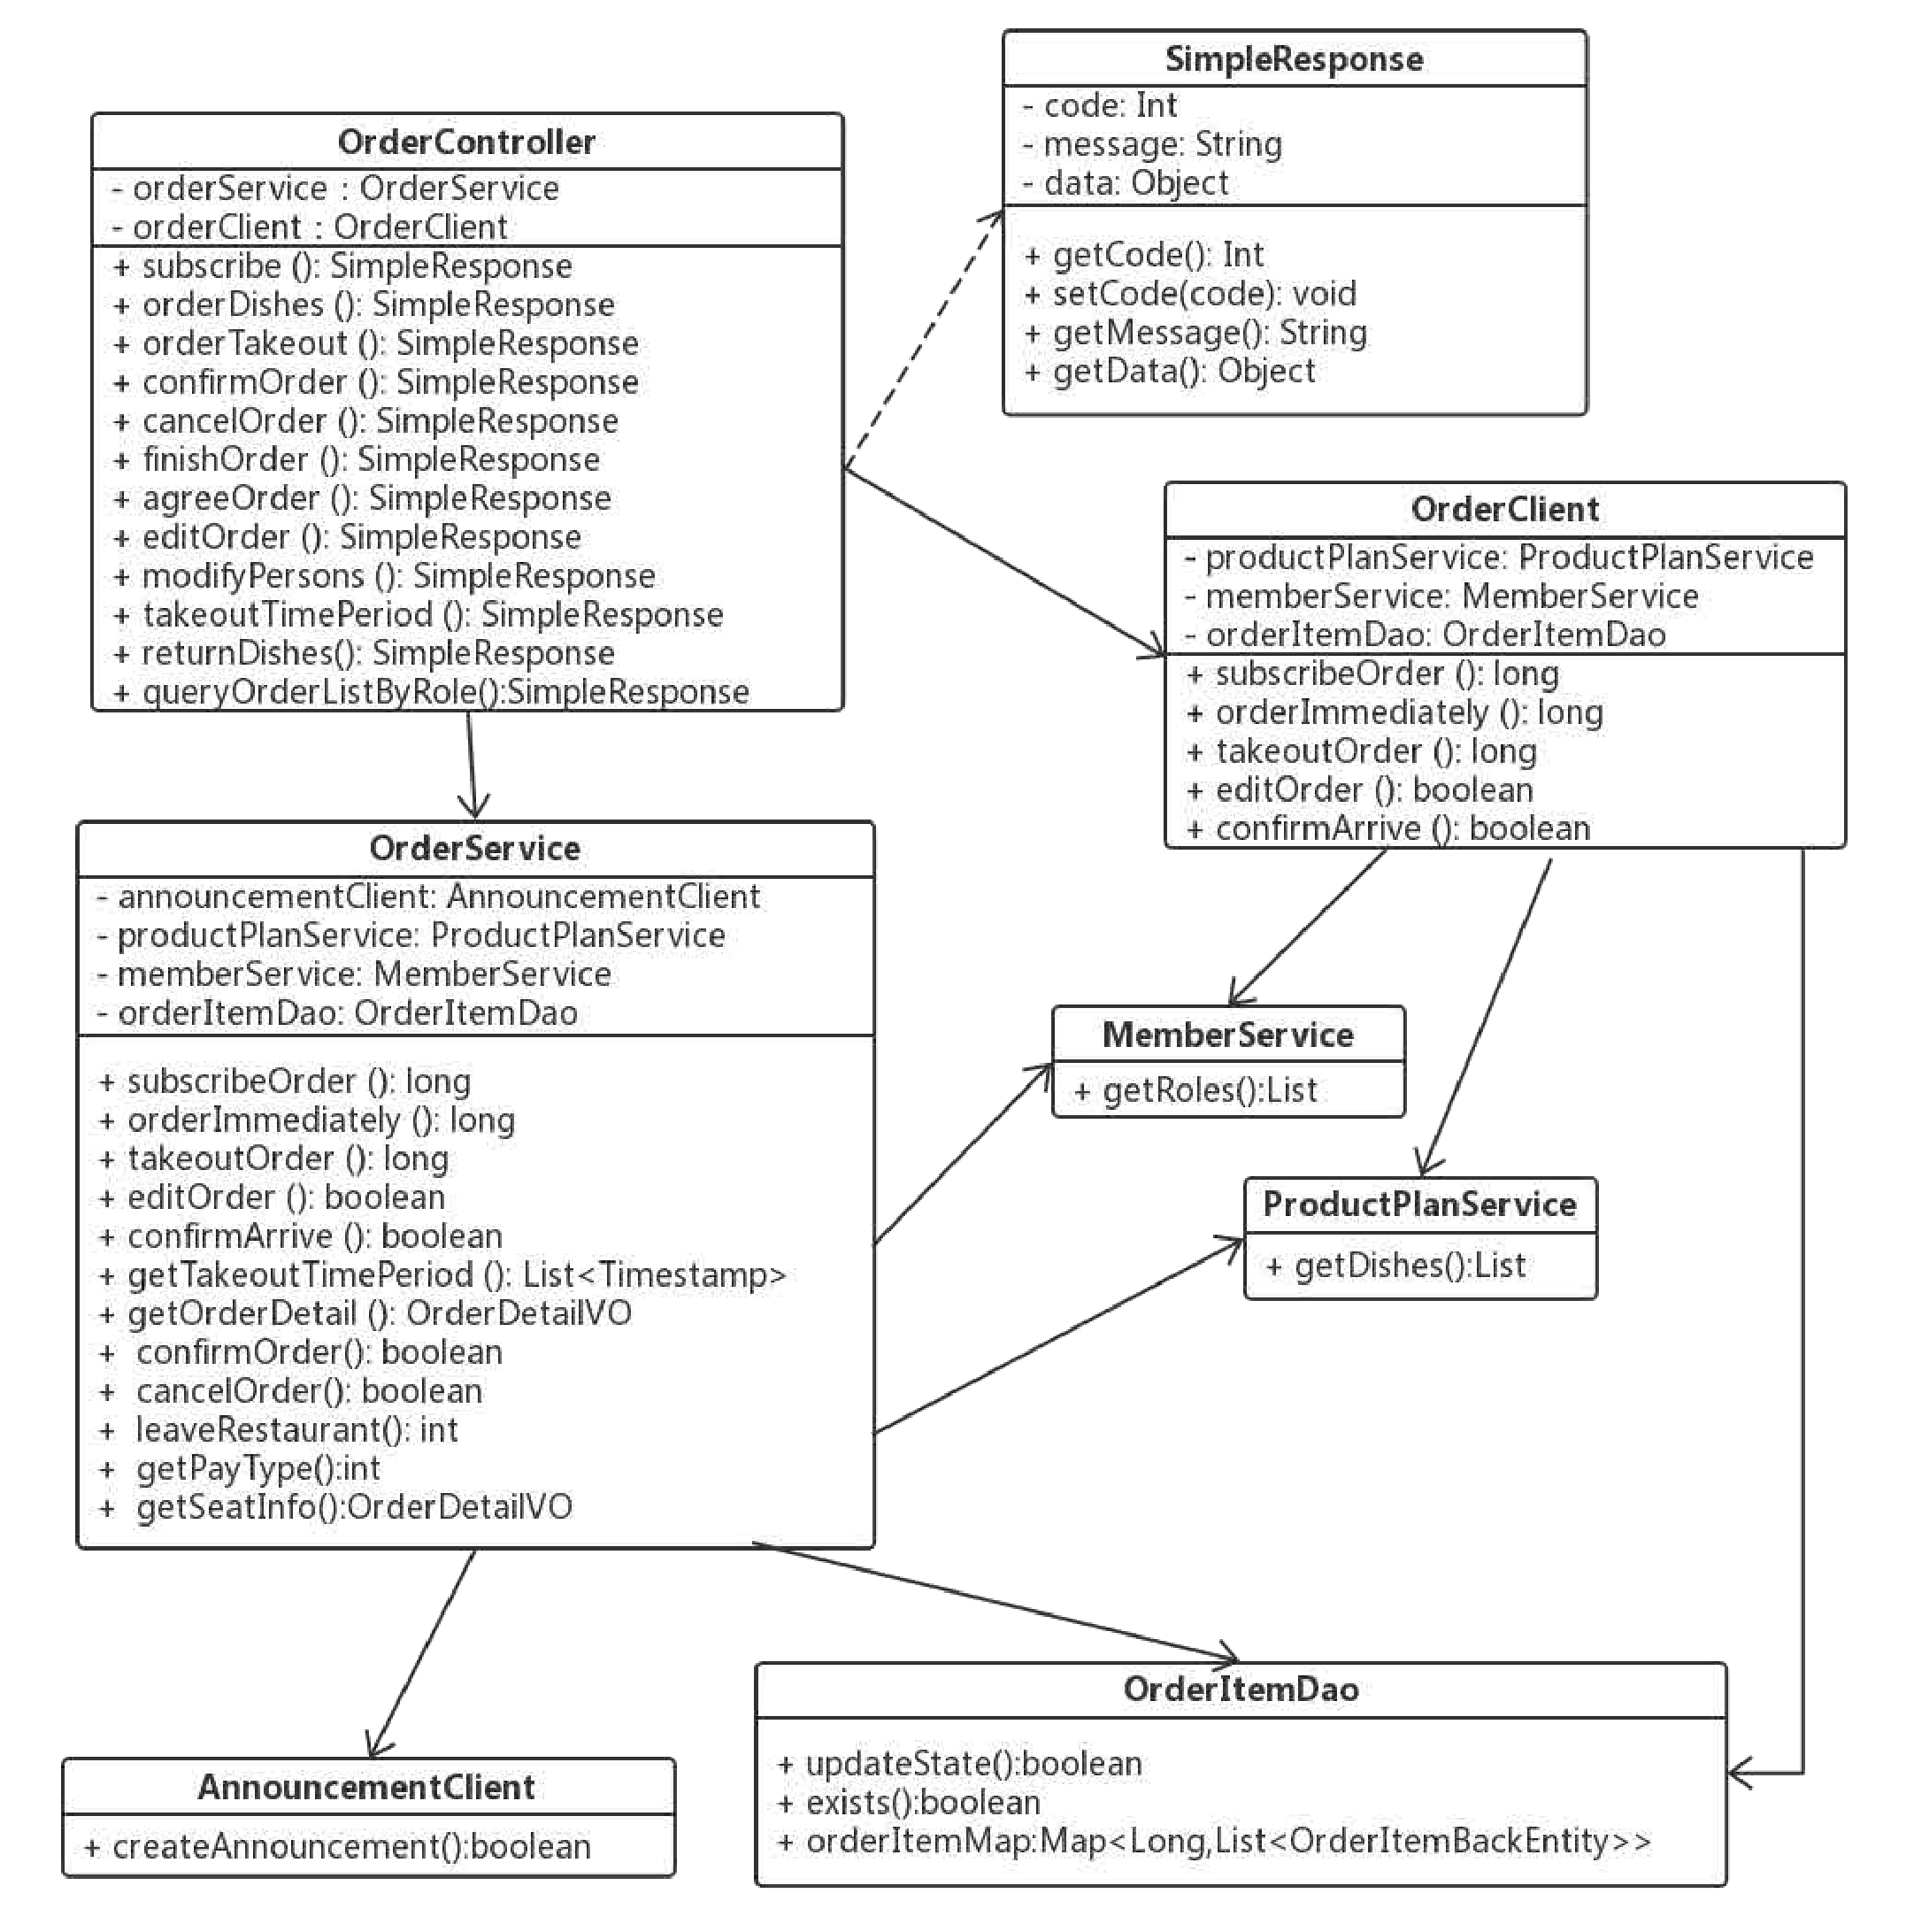
\includegraphics[width=5.2in]{FIGs/chapter4/order.pdf}
    \caption{订单发布模块关键类图}\label{fig_order}
\end{figure}

\begin{table}[htbp!]\footnotesize
    \centering
    \caption{订单发布模块涉及到的类及描述}
    \vspace{2mm}
    \begin{tabular}{clp{0.6\columnwidth}}
    \toprule
    \textbf{序号}&\textbf{名称}&\textbf{描述}\\
    \midrule 
    \textbf{1}& OrderController& 订单控制接口,直接传给前端的数据内容,包括顾客点单以及商家获取、操作订单发布内容。\\
    \hline
    \textbf{2}& OrderService& 订单服务接口,处理订单各类操作,包括提供到店点餐、预约点餐、外卖点餐、编辑订单、确认到店、取消订单等基础操作。\\
    \hline
    \textbf{3}& OrderClient& 订单客户端接口,获取顾客行为,顾客下单后的内容在这里获取。\\
    \hline
    \textbf{4}& SimpleResponse& 简单响应服务,获取接口状态、信息、数据等。\\
    \hline
    \textbf{5}& AnnouncementClient& 发布客户端接口,创建订单发布时需要调用该类创建、编辑等。\\
    \hline
    \textbf{6}& ProductPlanService& 生产计划服务接口,获取菜品详情、库存等内容。\\
    \hline
    \textbf{7}& MemberService& 用户服务接口,这里可以获取用户角色、基本信息、权限等。\\
    \hline
    \textbf{8}& OrderItemDao& 订单条目,更新订单状态、获取订单详情,与数据库交互。\\
    \bottomrule
    \end{tabular}
    \label{table:1List}
\end{table}

如表~\ref{table:1List}所示,订单发布模块主要关联到的java类有OrderController(订单控制接口)、OrderService(订单服务接口)、OrderClient(订单客户端接口)、SimpleResponse(简单响应服务)、AnnouncementClient(发布客户端接口)、ProductPlanService(生产计划服务接口)、MemberService(用户服务接口)、OrderItemDao(订单条目)。\\

\subsection{订单发布模块实现}

\begin{figure}[htbp!]
    \centering
    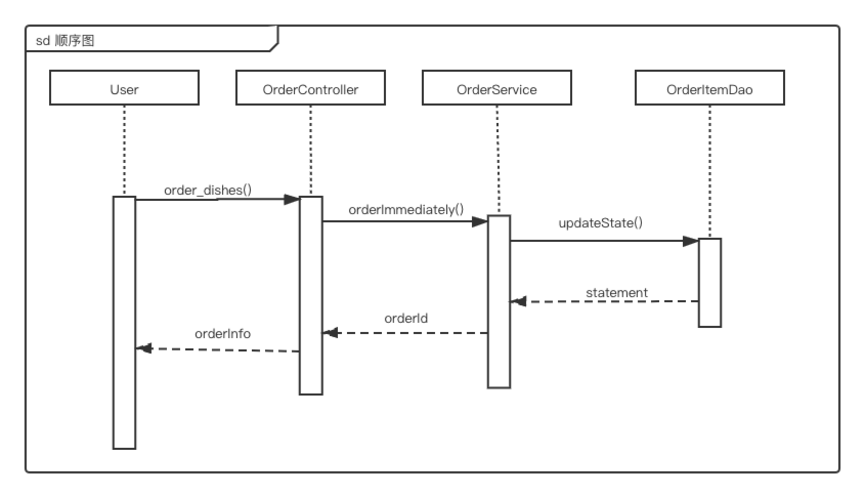
\includegraphics[width=5in]{FIGs/chapter4/order_time.pdf}
    \caption{用户到店点餐的时序图}\label{fig_order_time}
\end{figure}

如图~\ref{fig_order_time}所示,
这是用户到店点餐的过程,用户下单首先会调用OrderController的order\_dishes()方法创建订单,然后会调用OrderService中的orderImmediately()方法创建订单相关内容,在该方法中调用了generateAnnouncementOrder()方法创建订单发布,调用了OrderItemDao类中updateState()方法更新订单发布状态,最终返回给用户订单详情。

这是到店点餐的过程,预约点餐、外卖点餐与之类似,下单后需要根据下单类型创建相应的订单,运行不同任务以及改变其他模块的相关内容~\cite{jq2016}。如果是预约点餐,系统会将预约时间段的座位修改为已占用状态,允许用户在规定时间之前取消订单;如果是外卖点餐,系统会提醒商家确认接单,分配骑手送单等。

如图~\ref{fig_order_1}所示是生成订单发布的后端代码,用户下单后,需要在相应的餐厅事务下生成订单,记录其创建时间、公开性、创建内容并生成唯一的发布ID,记录下单用户、下单菜品以及订单状态。创建订单发布的同时调用了OrderClient类的createOrder()方法返回给用户订单详情。

\begin{figure}[htbp!]
    \centering
    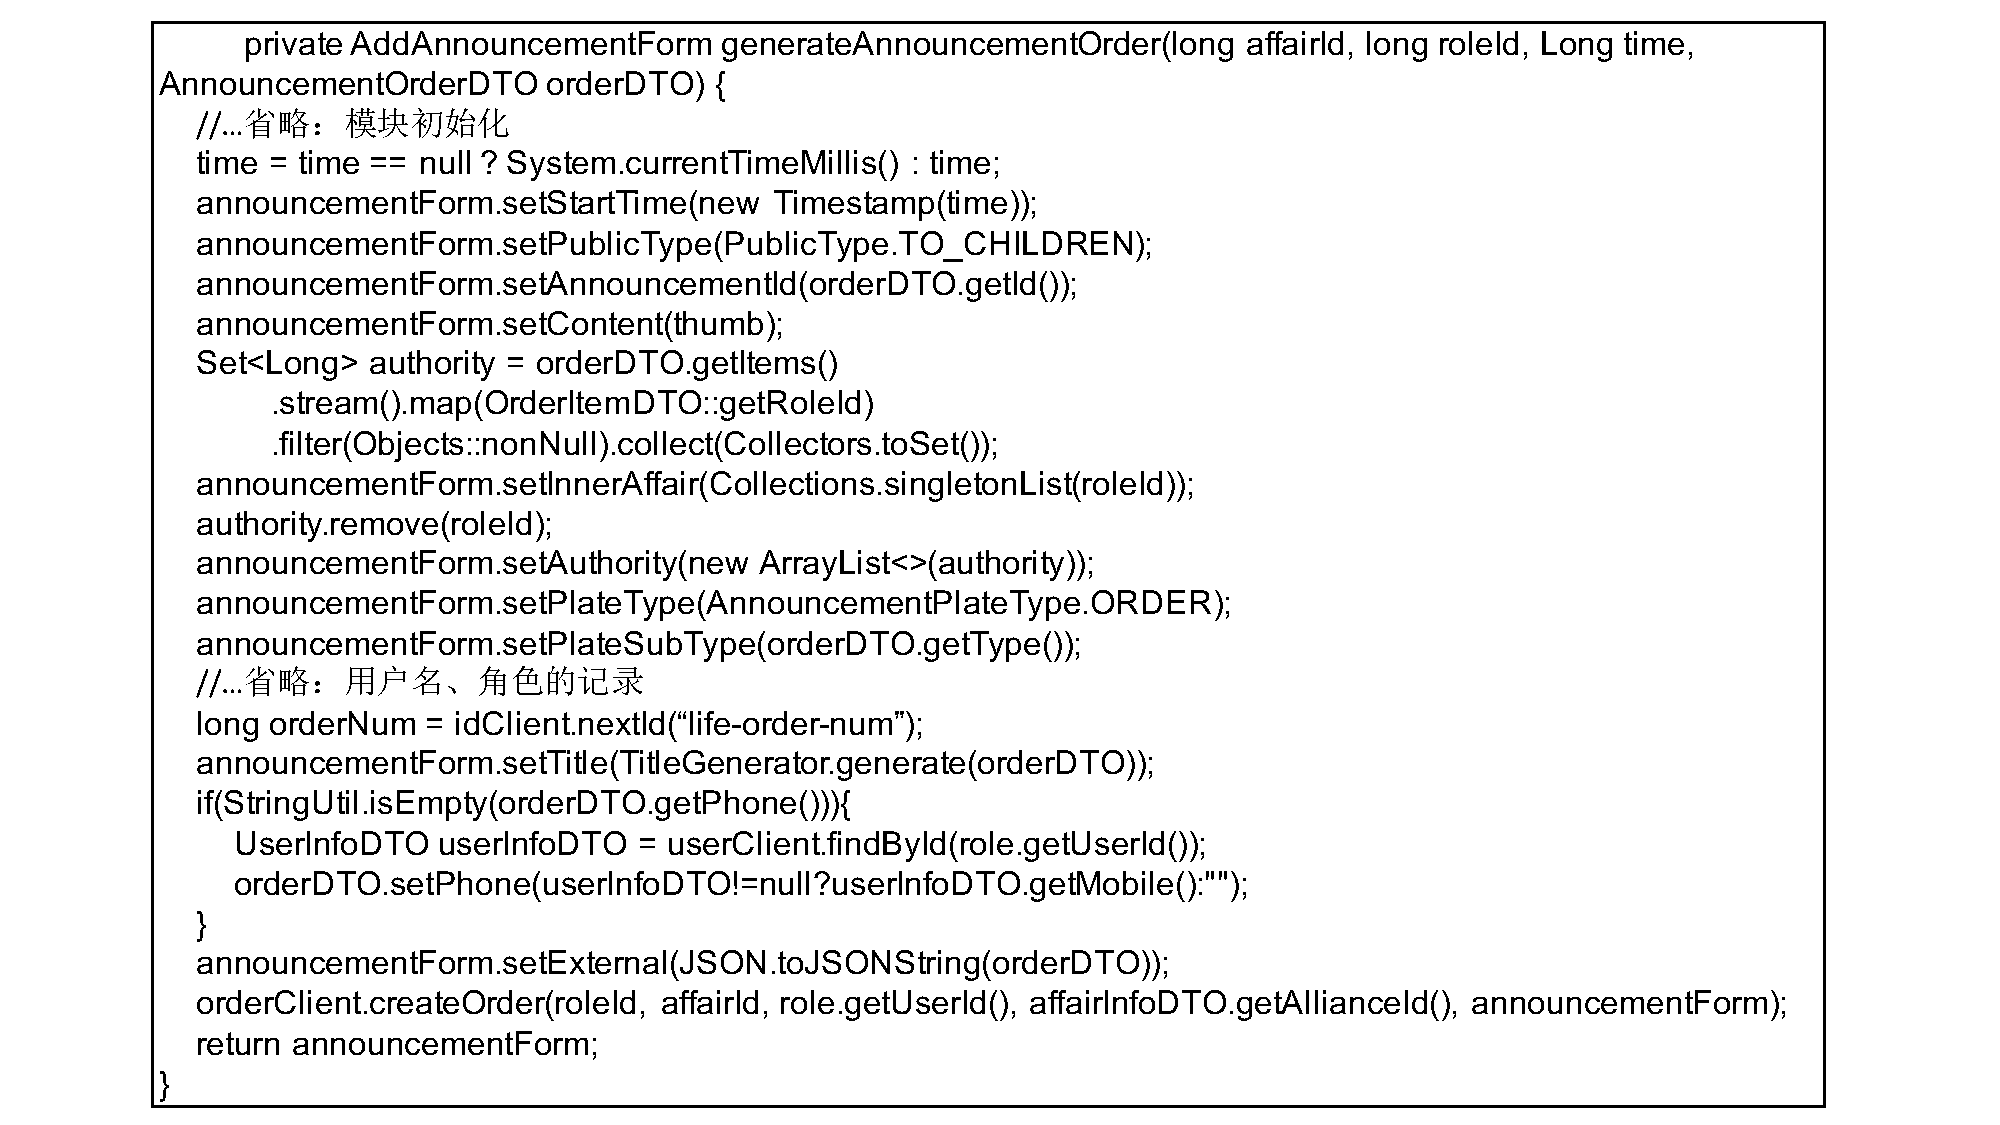
\includegraphics[width=\linewidth]{FIGs/chapter4/1.pdf}
    \caption{生成订单发布代码片段}\label{fig_order_1}
\end{figure}

\begin{figure}[htbp!]
    \centering
    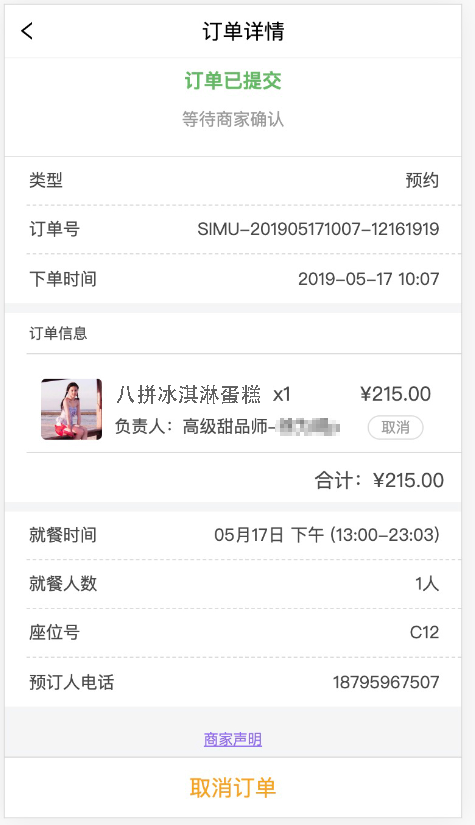
\includegraphics[width=2.5in]{FIGs/chapter4/order_view.pdf}
    \caption{顾客下单后的订单详情}\label{fig_order_view}
\end{figure}

\begin{figure}[htbp!]
    \centering
    \includegraphics[width=\linewidth]{FIGs/chapter4/order_view_all.pdf}
    \caption{订单发布详情和打印订单页面}\label{fig_order_detail}
\end{figure}

如图~\ref{fig_order_view}所示是顾客下单后的订单详情页面,这里以预约类型为例,内容包括订单类型(到店、预约、外卖)、唯一的订单号、下单时间、订单信息(菜品图片、名称、价格、厨师)、菜品合计价格、就餐时间、就餐人数、座位号、预订人电话等信息,顾客可以在商家确认之前取消订单,在菜品上菜之前取消某菜品。

如图~\ref{fig_order_detail}左侧所示是顾客下单后,商家在系统中查看到的相关订单发布的具体内容,这里以到店类型为例,包括订单类型(到店、预约、外卖)、订单名称、订单创建者、更新时间、唯一的订单号、座位号、顾客用餐时间、就餐人数、顾客到店时间、订单详情(产品、数量、总价值、状态、支付状态)、订单总金额等信息。商家可以对就餐人数进行修改,根据顾客需求对菜品做删减,当顾客支付完成后,商家点击确认离店即可完成该订单,还可以根据需要打印订单详情。

点击订单发布标题左侧的打印图标,即可看到如图~\ref{fig_order_detail}右侧所示的要打印订单的详情内容,这里以外卖类型为例,包括餐厅图片、名称、订单号、收货地址、联系电话(会加密保护顾客隐私)、配送时间、配送员、产品(名称、数量、总价值)、订单总金额、优惠金额、实付金额以及商家电话,点击打印即可打印该订单详情页。\\

% \begin{figure}[htbp!]
%     \centering
%     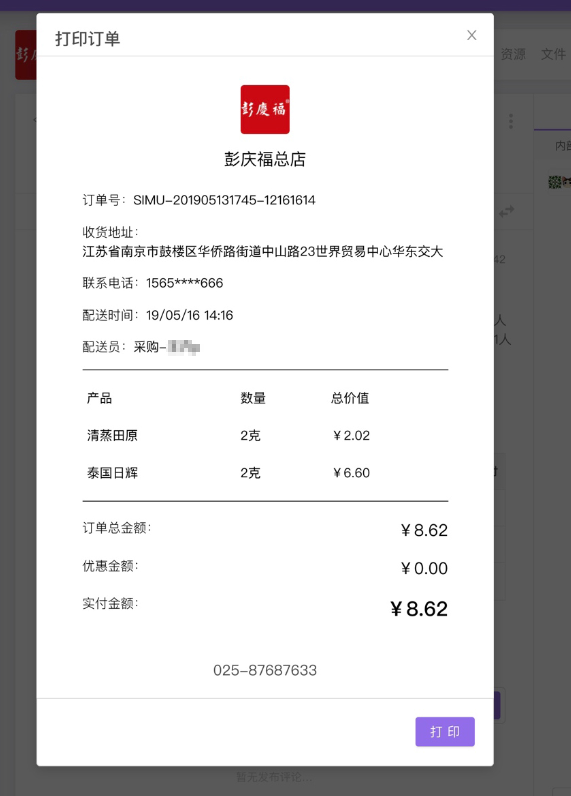
\includegraphics[width=2.5in]{FIGs/chapter4/order_print.pdf}
%     \caption{打印订单}\label{fig_order_print}
% \end{figure}

\section{支付模块}
\subsection{支付模块介绍}
支付模块主要负责处理顾客支付时的支付安全和第三方支付,包括微信支付、支付宝支付等,它依赖于订单发布。对于提交后的订单,顾客支付时系统会调用微信或者支付宝支付接口完成订单支付工作。\\

\subsection{支付模块详细设计}
\begin{figure}[htbp!]
    \centering
    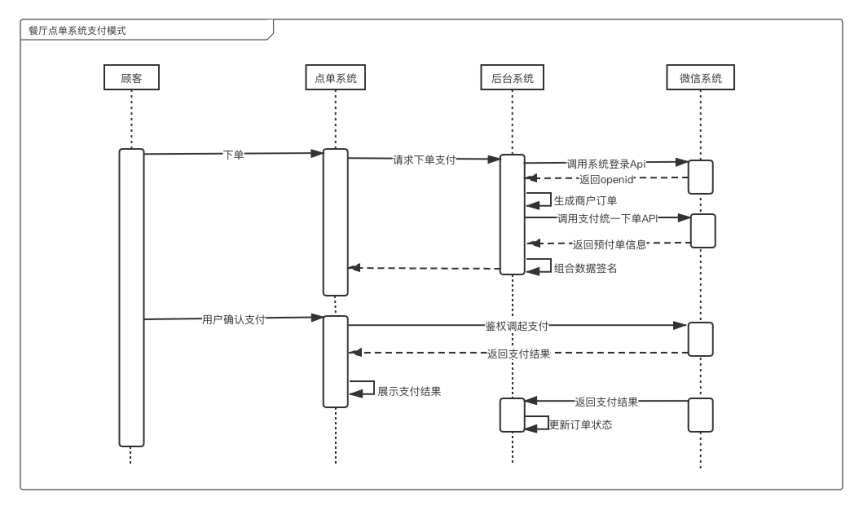
\includegraphics[width=5in]{FIGs/chapter4/pay_time.pdf}
    \caption{点单系统支付模块时序图}\label{fig_pay_time}
\end{figure}

以微信支付为例,微信支付主要分为两种——普通模式和服务商模式,本系统选择普通模式,商家需要申请一个微信公众号绑定店铺,认证通过并且需要成功申请到微信支付功能。此时,商家会在平台中收到唯一的商户号、商户平台密码等内容,可以用于微信支付。开发者可以申请个人的appid以及mch\_id,拥有唯一的appid后可以进行微信公众号内程序的开发,使用微信支付提供给开发者的开放接口来对用户提供相应服务~\cite{fff}。

微信支付功能的SDK,其中包括WxPay.Api.php(微信支付SDK的接口)、WxPay.Config.php(微信支付的配置文件)、WxPay.Data.php(微信支付中要用到的基本参数对象)、WxPay.Notify.php(接受回调信息的处理类)、WxPay.Exception.php(处理错误异常类)五个主要文件~\cite{czz2018}。如图~\ref{fig_pay_time}所示是餐厅点单系统支付模块的时序图,顾客下单后首先会将订单详情发送到后台服务器,由服务器传递参数openid调用微信平台提供的统一下单API,生成预付单并返回到系统的后台服务器,系统将签名后内容和预付单参数信息返还给前端,前端收到信息后调用wx.requestPayment,提交到微信平台,若验证通过则会展示商家的支付二维码界面,顾客扫描二维码即可支付订单。
顾客在公众号内进入系统,选定菜品加入购物车下单。系统生成订单后,会通过wx.navigateTo API跳转到微信的支付模块,调用QRCodePay类实现扫码支付功能,支付成功后微信会返回给顾客相应的支付结果。\\

\subsection{支付模块实现}
\begin{figure}[htbp!]
    \centering
    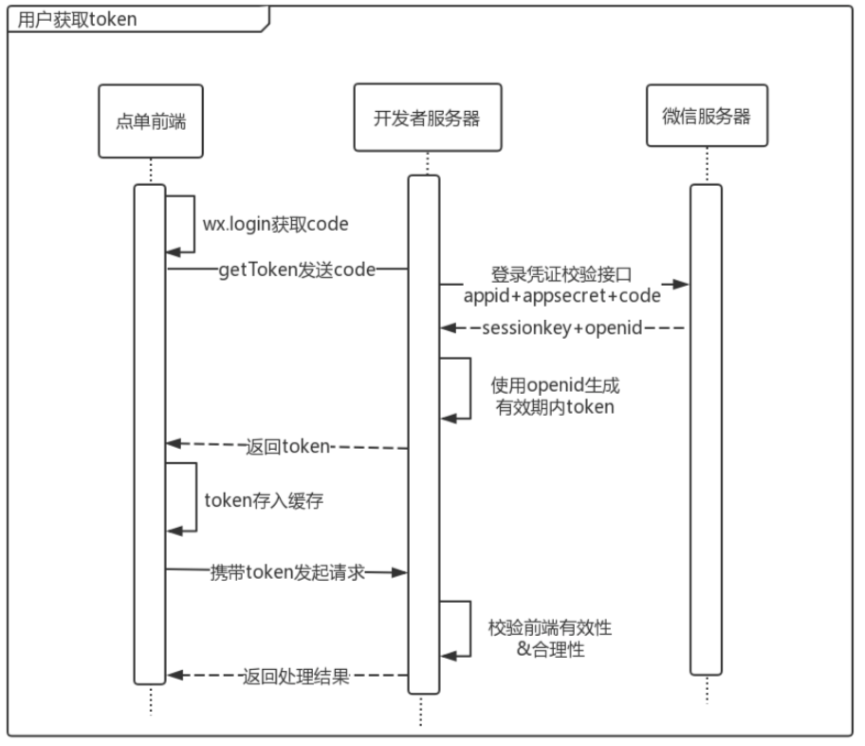
\includegraphics[width=4in]{FIGs/chapter4/pay_token.pdf}
    \caption{用户获取token时序图}\label{fig_pay_token}
\end{figure}

如图~\ref{fig_pay_token}所示,为了验证用户信息,保证支付安全,用户登录时会收到一个code码,后台服务器通过getToken接口把用户信息、code码等内容发送到微信平台中,再由微信平台服务器返回openid以及session\_key参数给后台服务器~\cite{lby2019}。
后台服务器需要保存openid,并以此作为验证用户的唯一标志,将其处理加工成一定时间段内有效的token令牌,返回给用户。

用户访问支付接口时,开发者服务器会先对token和openid进行验证,校验通过后,后端会把处理结果返回给前端,用户可以进行相应的后续操作。这样不光保证了支付过程的安全性,而且保护了用户隐私,防止第三方恶意入侵。

\begin{figure}[htbp!]
    \centering
    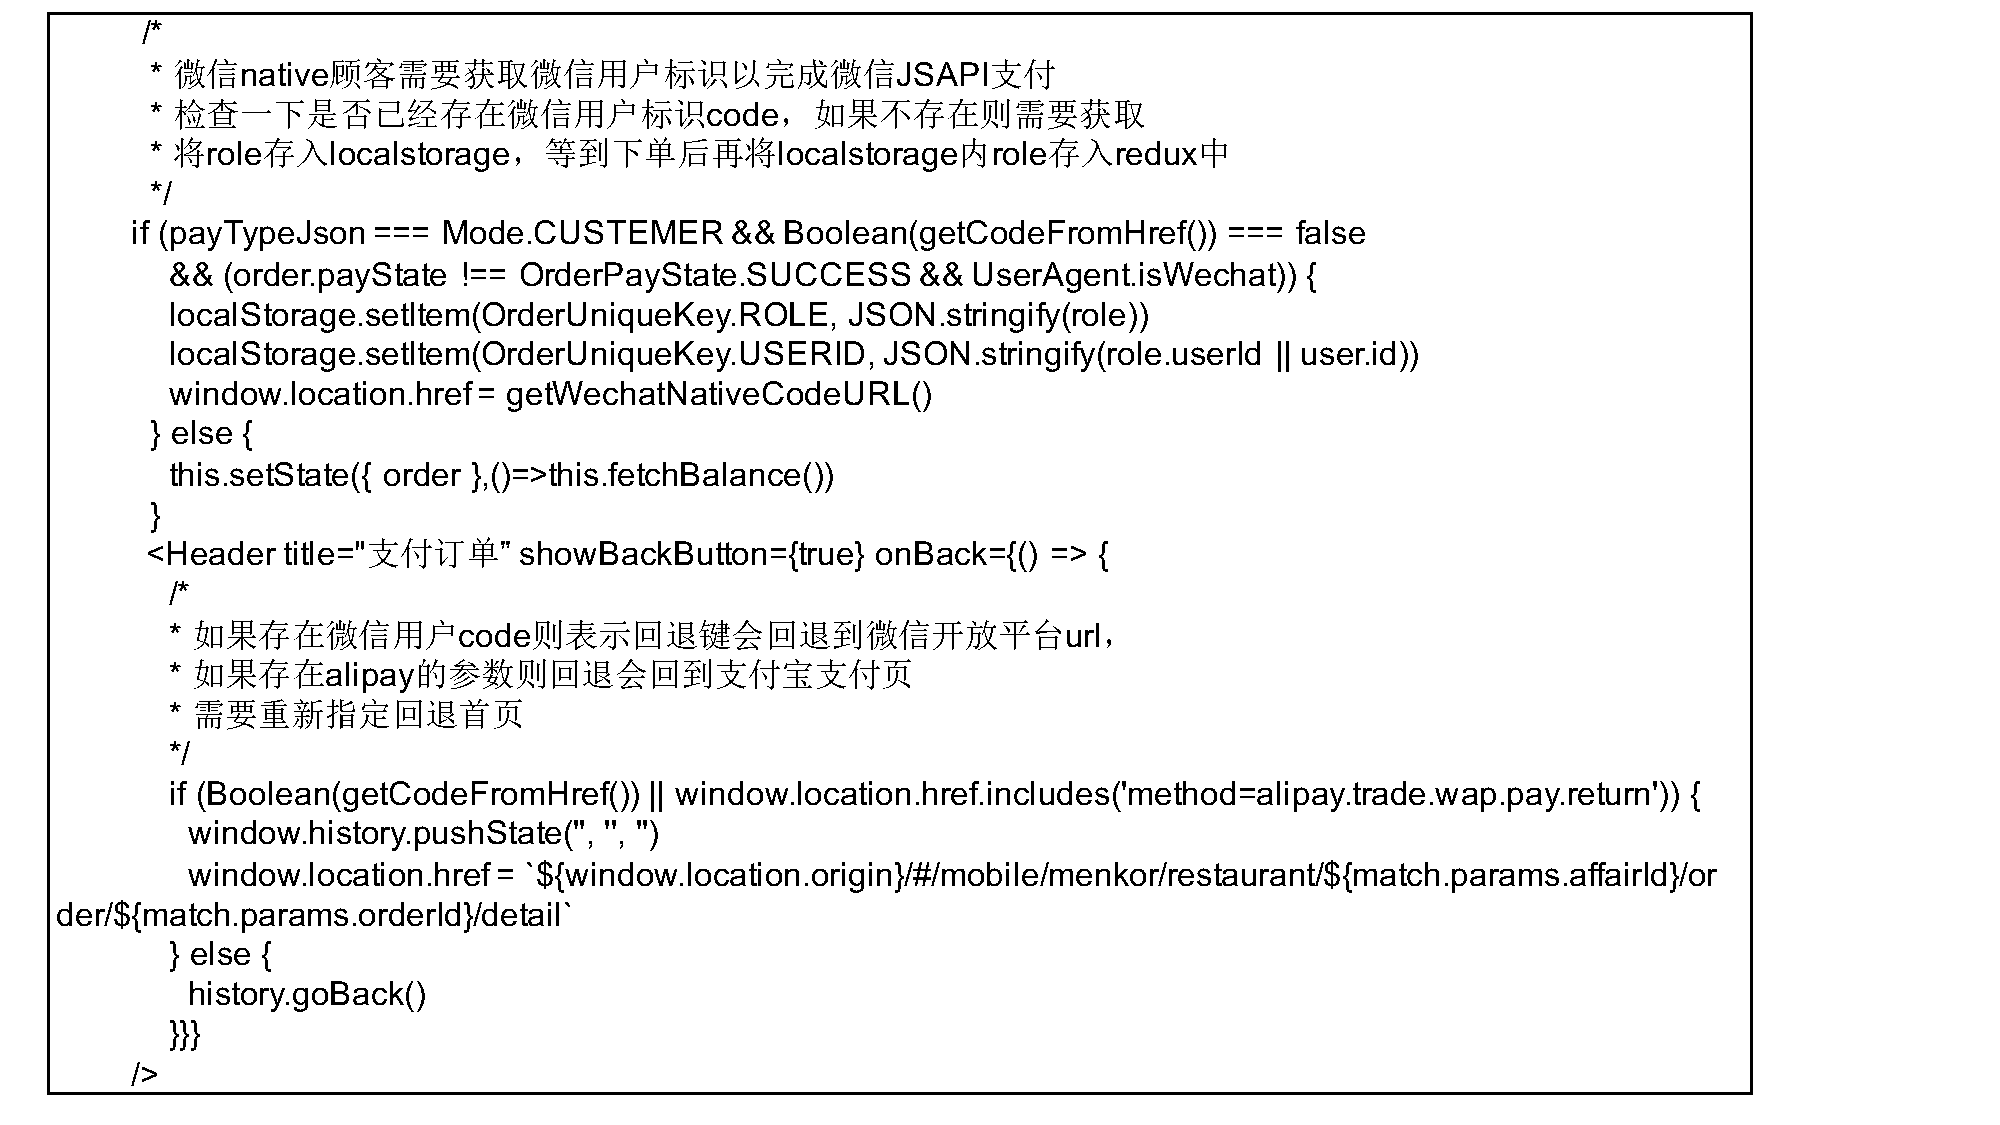
\includegraphics[width=\linewidth]{FIGs/chapter4/2.pdf}
    \caption{判断微信支付代码片段}\label{fig_pay_2}
\end{figure}

系统的线上支付操作一共有两种方式,一种是用户直接点击付款,后端调用相应支付方式的链接以供后续操作;一种是商家出示付款码,用户扫码支付。

如图~\ref{fig_pay_2}所示是前端OrderPaymentContainer订单支付类获取微信用户标识的代码片段,在进入未付款订单前首先判断用户是否为微信用户,如果是则需要获取微信用户标识,如果已经有code码则无须再次获取。系统在回退页上面做了逻辑控制,微信客户端用户与支付宝客户端用户在支付完成后,点击订单界面的返回按钮会回到相对应平台的界面。

为了防止支付完成后,微信刷新页面将缓存内的用户信息清除掉,系统使用了localstorage暂时存储用户信息,等到支付完成后再将其存进Redux的Store内,保持用户数据的实时性与准确性~\cite{mys2019}。

支付时同样可以使用商家收款码扫码收款或者现金结账,如图~\ref{fig_pay_3}所示前端ReceiptContainer收款类商家收款代码片段,支持用户使用现金、微信支付、支付宝支付,如果使用现金支付,系统会显示需要支付的金额,商家需要记录抹零后实际收到的金额,保证数据平衡。如果使用微信或者支付宝支付时,系统将返回商家收款码,用户直接扫码即可付款,支付完成3秒后付款码会自动关闭,订单状态更新。\\

\begin{figure}[htbp!]
    \centering
    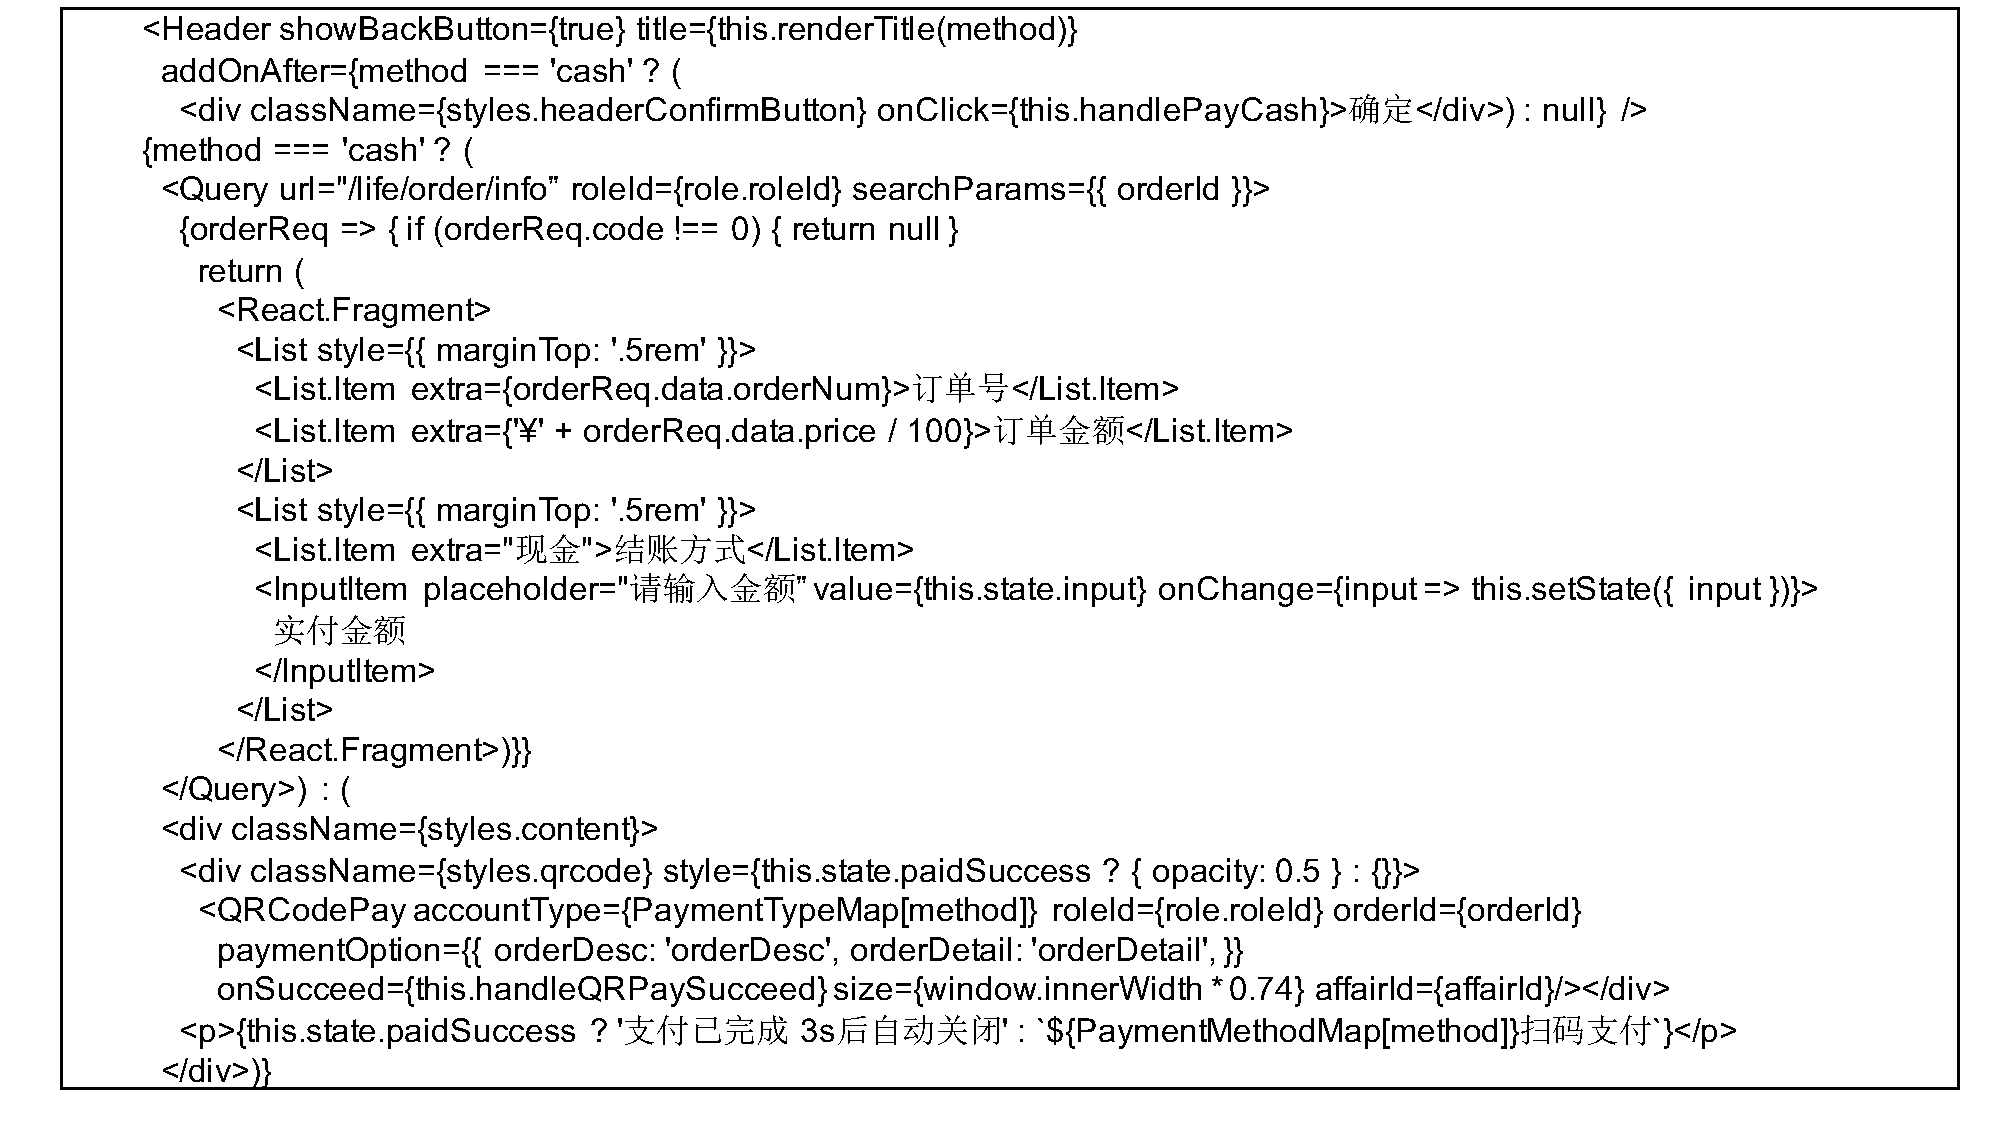
\includegraphics[width=\linewidth]{FIGs/chapter4/3.pdf}
    \caption{商家收款代码片段}\label{fig_pay_3}
\end{figure}

\section{用户管理模块}
\subsection{用户管理模块介绍}
用户管理模块分为两部分:商家部分主要管理餐厅简介、地址、联系电话等信息;顾客部分主要管理账户角色(同一个账号的不同角色可能会对应不同的折扣,使用不同角色登录所看到的订单列表、余额等内容也是不同的)、用户姓名、手机号、配送地址等信息。\\

\subsection{用户管理模块详细设计}
\begin{figure}[htbp!]
    \centering
    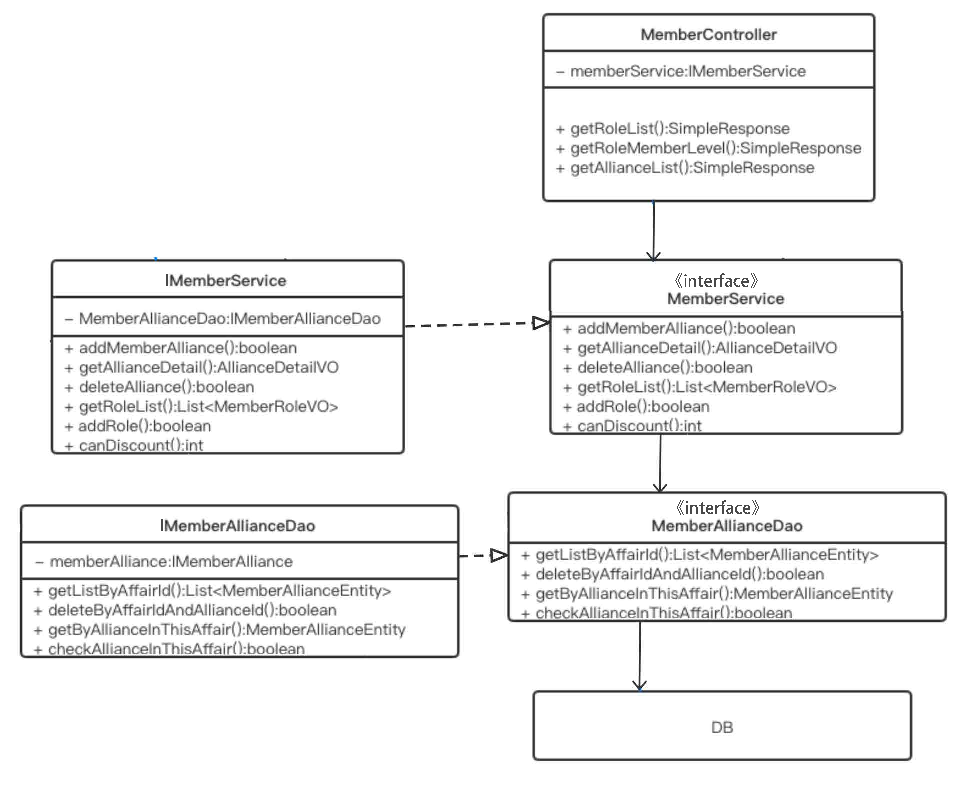
\includegraphics[width=\linewidth]{FIGs/chapter4/user.pdf}
    \caption{用户管理模块类图}\label{fig_user}
\end{figure}

如图~\ref{fig_user}所示是用户管理模块的类图,这里涉及的几个类分别是:MemberController类是用户控制接口,可以获取用户的角色列表、获取角色会员等级、获取餐厅名称等;MemberService类是用户服务接口,主要提供添加商家店铺、获取餐厅详情、删除餐厅、获取角色列表、判断会员是否享受折扣等服务,其中IMemberService是它的实现类;MemberAllianceDao类是用户服务的Dao层,主要负责与数据库交互,提供基本的用户数据,其中IMemberAllianceDao是它的实现类~\cite{zzz2019}。

在顾客点单平台中,可以点击用户头像进入到个人中心,查看用户头像、用户名、账号、当前角色等内容。
\\

\subsection{用户管理模块实现}
如图~\ref{fig_user_4}是判断顾客当前角色是否享受折扣并且返回相应折扣的方法,顾客所在的分组如果享受折扣,会返回该角色拥有的折扣度,否则直接返回100表示没有折扣。

\begin{figure}[htbp!]
    \centering
    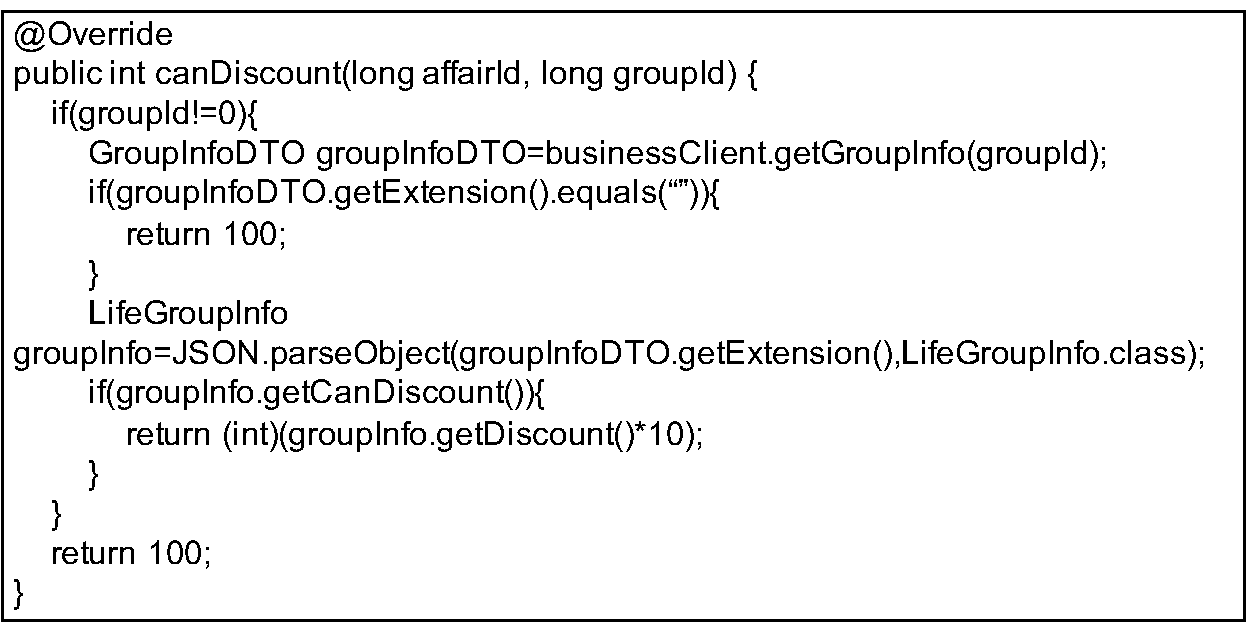
\includegraphics[width=4.4in]{FIGs/chapter4/4.pdf}
    \caption{是否打折的代码片段}\label{fig_user_4}
\end{figure}

如图~\ref{fig_user_5}所示是获取用户所有角色列表的代码片段,通过当前的用户ID与所在餐厅ID去获取当前用户在该餐厅内的所有角色。需要先获取用户的所有角色,再通过餐厅ID筛选当前可选角色,去除重复角色后,将用户本身会员折扣与分组内的会员折扣对比,取最大折扣值返回给相应角色,并按照折扣力度降序排列,返回角色列表。

\begin{figure}[htbp!]
    \centering
    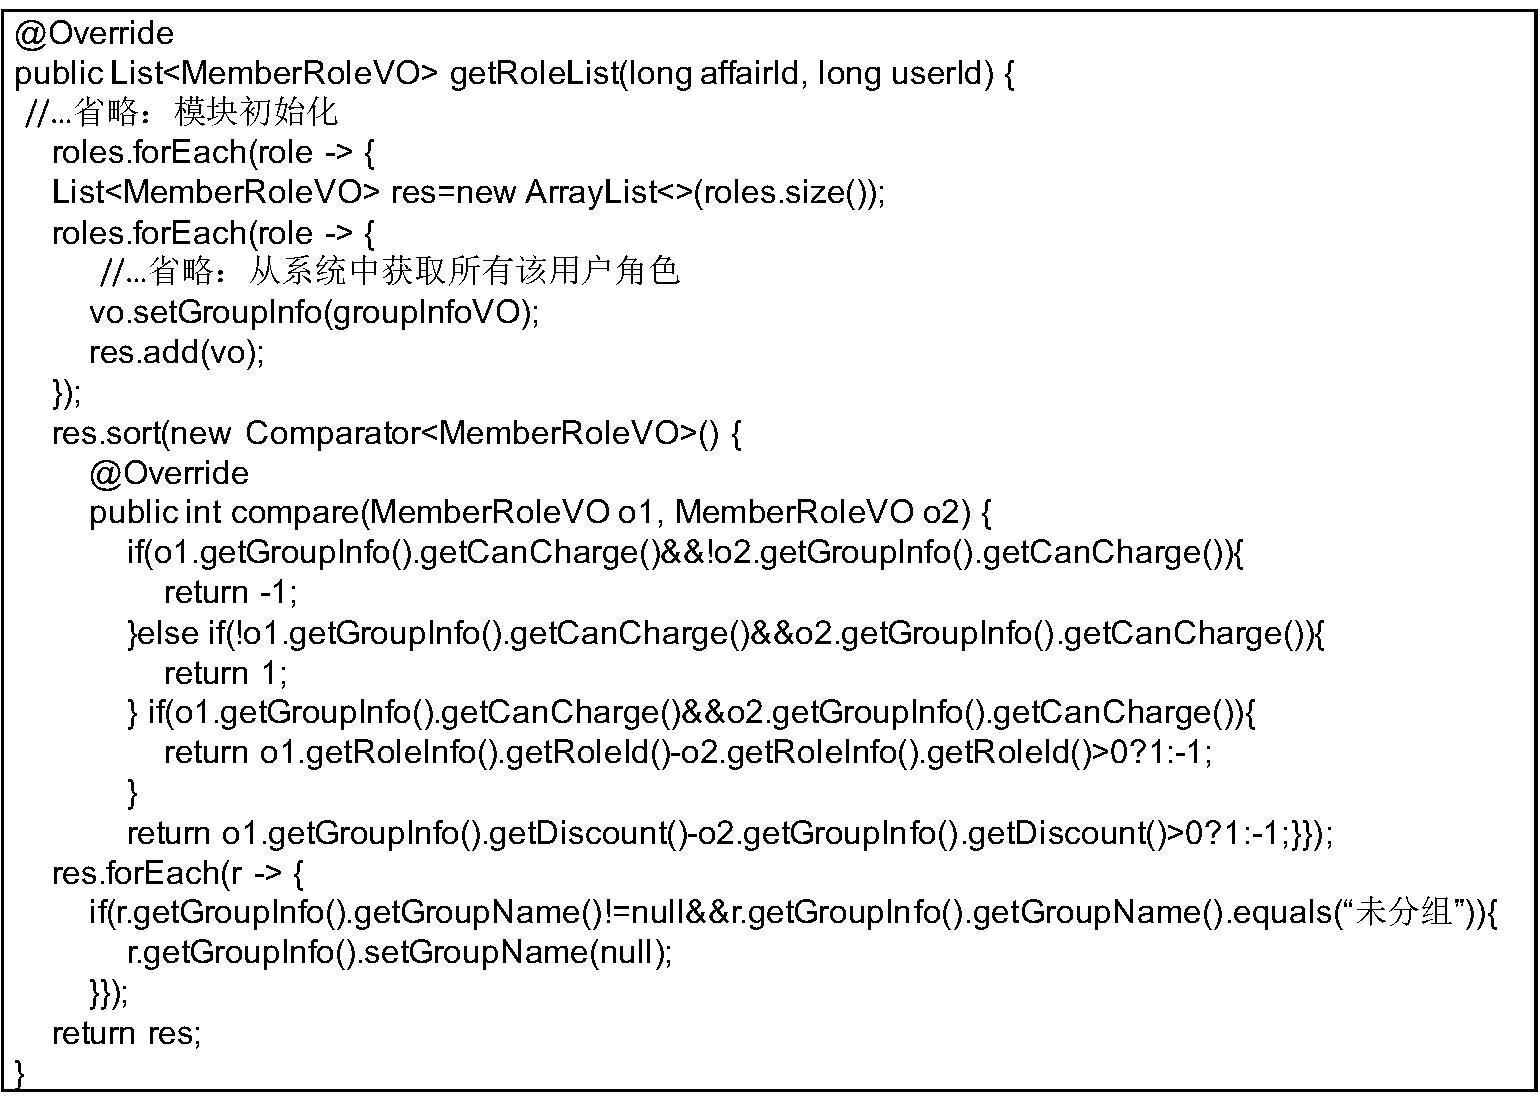
\includegraphics[width=5.5in]{FIGs/chapter4/5.pdf}
    \caption{获取用户所有的角色列表代码片段}\label{fig_user_5}
\end{figure}

用户可以在如图~\ref{fig_user_role_view}左侧所示的个人中心中,查看当前用户的账户、头像、角色,点击当前角色可以选择切换角色。如图~\ref{fig_user_role_view}右侧所示是当前顾客的角色列表(按照会员折扣降序排列),默认角色为最大折扣角色。

\begin{figure}[htbp!]
    \centering
    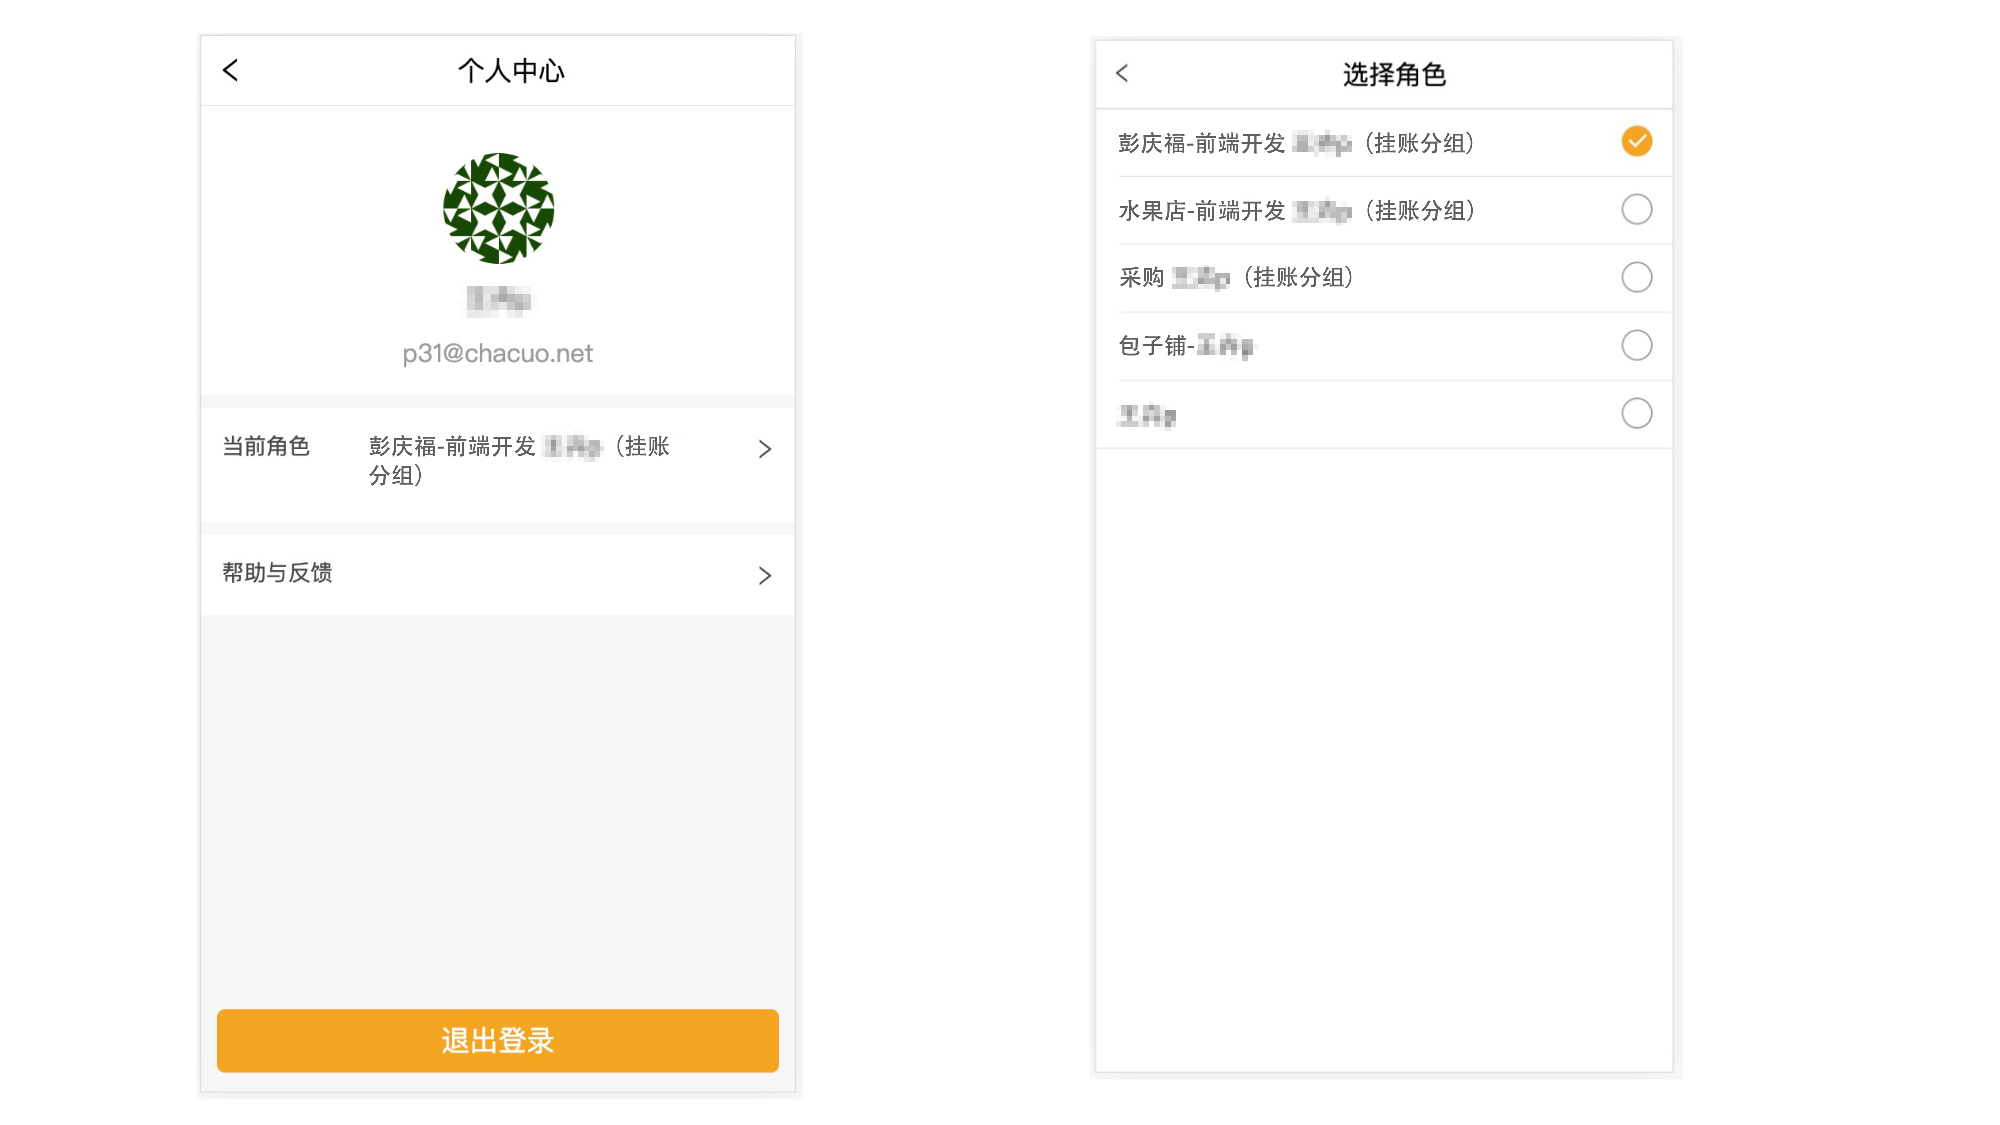
\includegraphics[width=\linewidth]{FIGs/chapter4/user_role_view.pdf}
    \caption{个人中心}\label{fig_user_role_view}
\end{figure}

\section{统计报表模块}
\subsection{统计报表模块介绍}
统计报表模块主要负责收集、整合各报表的信息,对外提供查看日报表、月报表、菜品的进销存日报表、原材料的进销存日报表,下载各报表的服务,为出品发布模块提供下载采购需求的接口。

商家可以在报表内筛选查看每日、每周、每月、每年的菜品统计、销售统计、收支等内容,便于对之后的菜品库存、经营策略、每日配餐组合等内容做出相应调整~\cite{dwh2019}。\\

\subsection{统计报表模块详细设计}
如图~\ref{fig_table}所示是统计报表模块的类图,这里涉及的几个类分别是:ReportFormController类是报表控制接口,可以查看并下载简单报表、复杂日报表、复杂月报表、菜品进销存报表、原材料进销存报表等;ReportFormService类是报表服务接口,主要提供获取简单报表、复杂日报表、复杂月报表等服务,其中IReportFormService是它的实现类;OrderItemDao类前面有介绍过,这里主要用于提供订单详情,其中IOrderItemDao是它的实现类。

\begin{figure}[htbp!]
    \centering
    \includegraphics[width=5.3in]{FIGs/chapter4/table.pdf}
    \caption{统计报表模块类图}\label{fig_table}
\end{figure}

\subsection{统计报表模块实现}
\begin{figure}[htbp!]
    \centering
    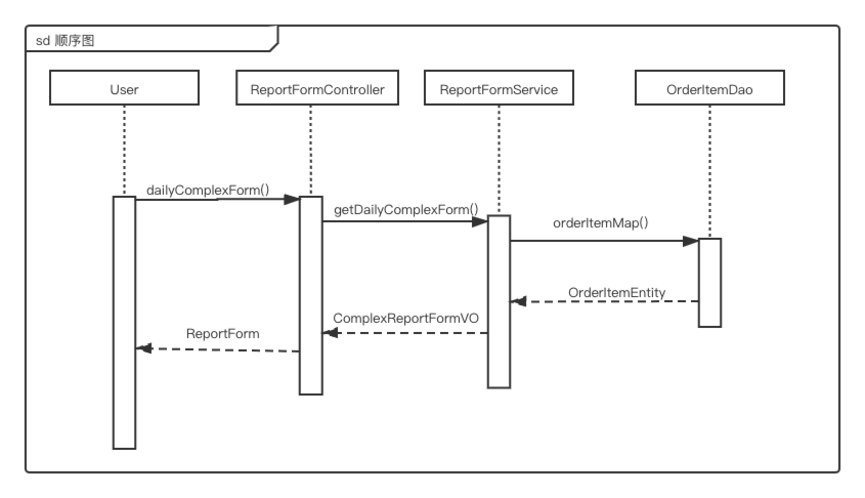
\includegraphics[width=5in]{FIGs/chapter4/table_time.pdf}
    \caption{查看日报表的时序图}\label{fig_table_time}
\end{figure}

如图~\ref{fig_table_time}所示是ReportFormController类dailyComplexForm方法的执行时序图,用户点击查看报表,会先调用控制层的查看日报表方法,接着调用ReportFormService类中的getComplexForm方法获取复杂的日报表,这里需要依赖到订单发布模块中OrderItemDao类的orderItemMap方法得到当日订单详情,经过处理返回给上一级,逐步获取、解析并处理好报表信息后,返回报表数据列表给用户。

\begin{figure}[htbp!]
    \centering
    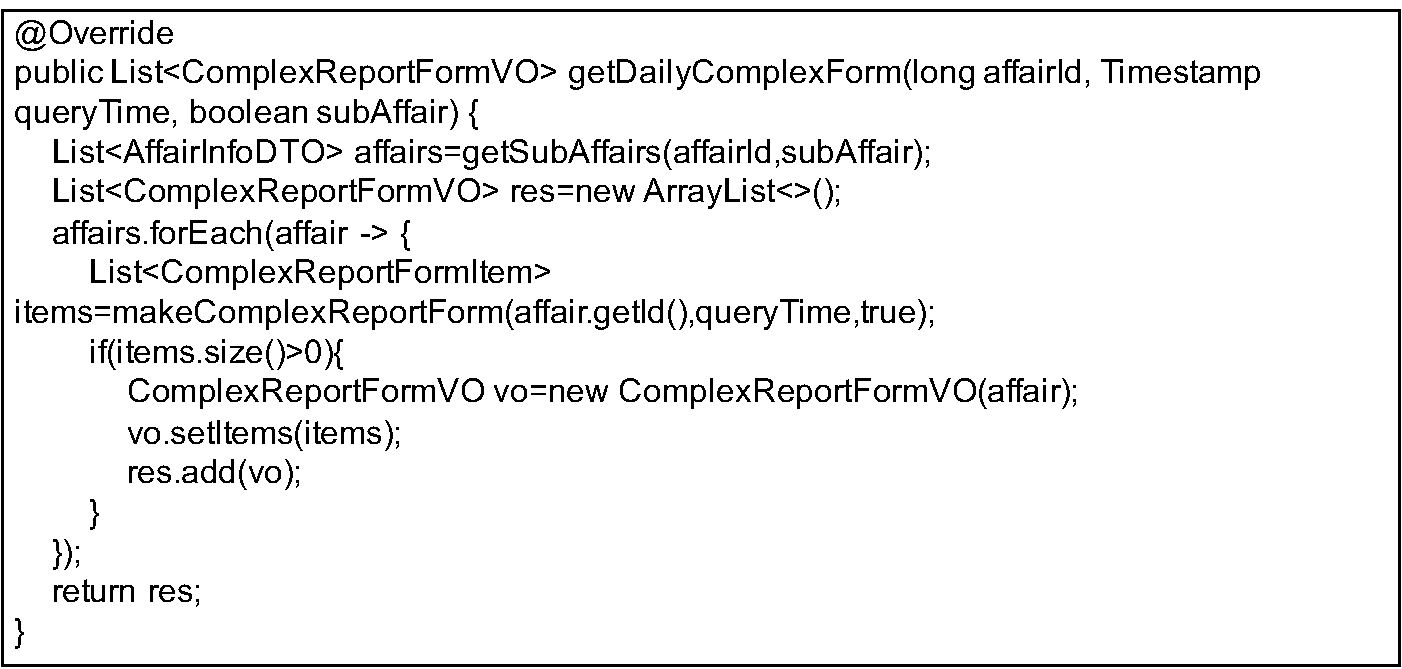
\includegraphics[width=5in]{FIGs/chapter4/6.pdf}
    \caption{ReportFormService类getComplexForm方法代码}\label{fig_table_6}
\end{figure}

统计报表部分实现的代码如图~\ref{fig_table_6}所示,其中调用了私有方法makeComplexReportForm返回报表内容,该方法根据传入的时间参数返回该时间内的报表,根据订单类型(到店、预约、外卖)创建不同的报表内容包括订单折扣、总价、实际收入、支付方式等多种内容~\cite{lz2019}。根据传入的餐厅ID来筛选该餐厅下所有的日报表信息(如果该餐厅为连锁餐厅,则可以在总店查看包括总店、分店在内的所有餐厅报表信息)。

\begin{figure}[htbp!]
    \centering
    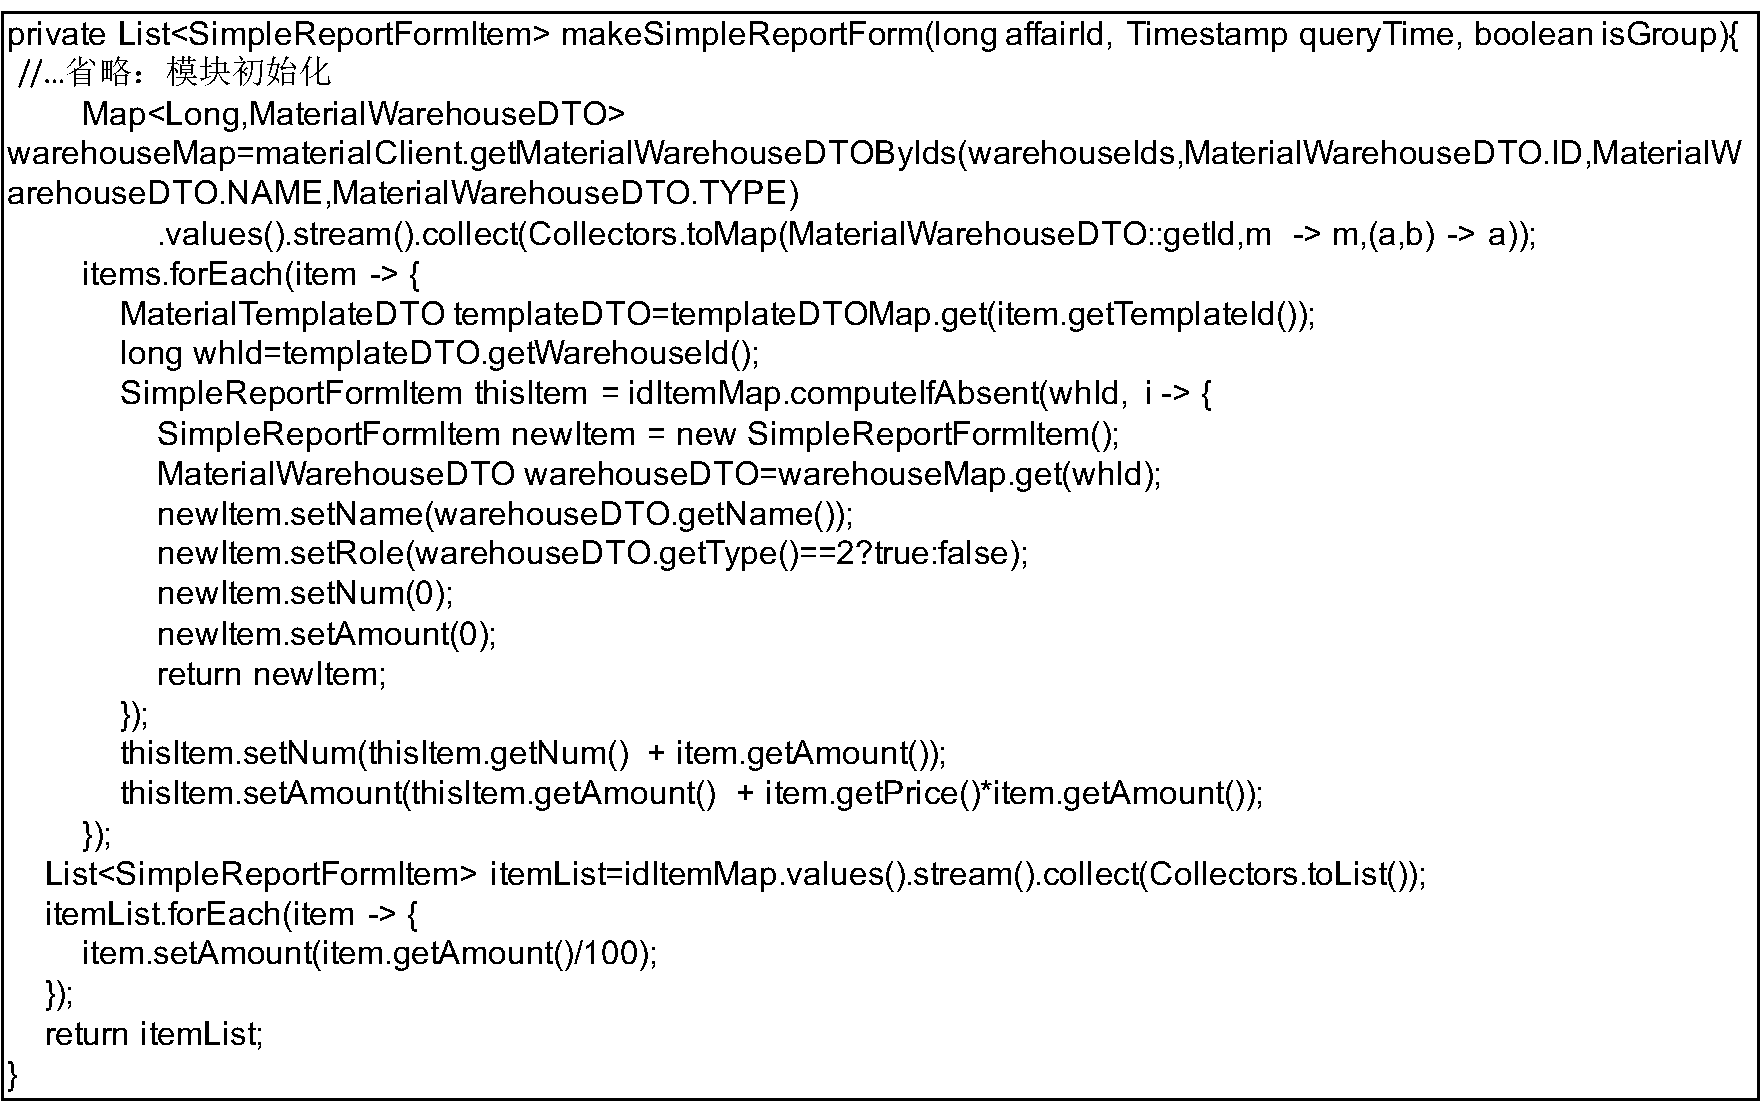
\includegraphics[width=\linewidth]{FIGs/chapter4/7.pdf}
    \caption{ReportFormService类中makeSimpleReportForm方法代码}\label{fig_table_7}
\end{figure}

\begin{figure}[htbp!]
    \centering
    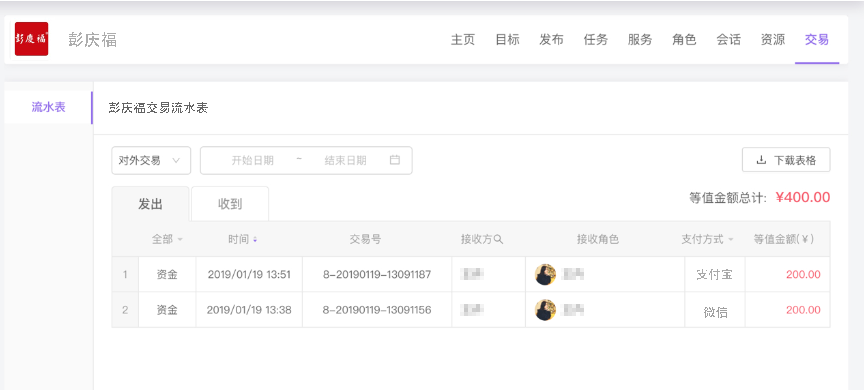
\includegraphics[width=\linewidth]{FIGs/chapter4/table_figure.pdf}
    \caption{简单报表}\label{fig_table_figure}
\end{figure}

如图~\ref{fig_table_7}所示是ReportFormService类中makeSimpleReportForm方法的实现代码,该方法用于获取简单报表,不需要区分订单类型,通过日期来筛选订单并且创建包括用户名、用户角色、菜品编号、菜品数量、价格等的简单报表,计算订单的总金额。

如图~\ref{fig_table_figure}所示是简单报表的前端界面,可以根据交易类型、起止时间来筛选查看不同的报表内容,报表内容主要包括类型、时间、交易号、接收方信息、支付方式以及金额等内容,可以点击下载表格将报表内容存储到本地。\\

\section{座位管理模块}
\subsection{座位管理模块介绍}
座位管理模块主要处理与座位库以及座位有关的操作,对外提供管理座位库的平面视角、卡片视角以及时间轴视角,对座位进行增删改查、更改座位状态、检查是否有重名座位、获取座位信息、座位二维码、座位状态等接口,同时还负责向订单发布模块提供与订单绑定的座位信息等接口。\\

\subsection{座位管理模块详细设计}

\begin{figure}[htbp!]
    \centering
    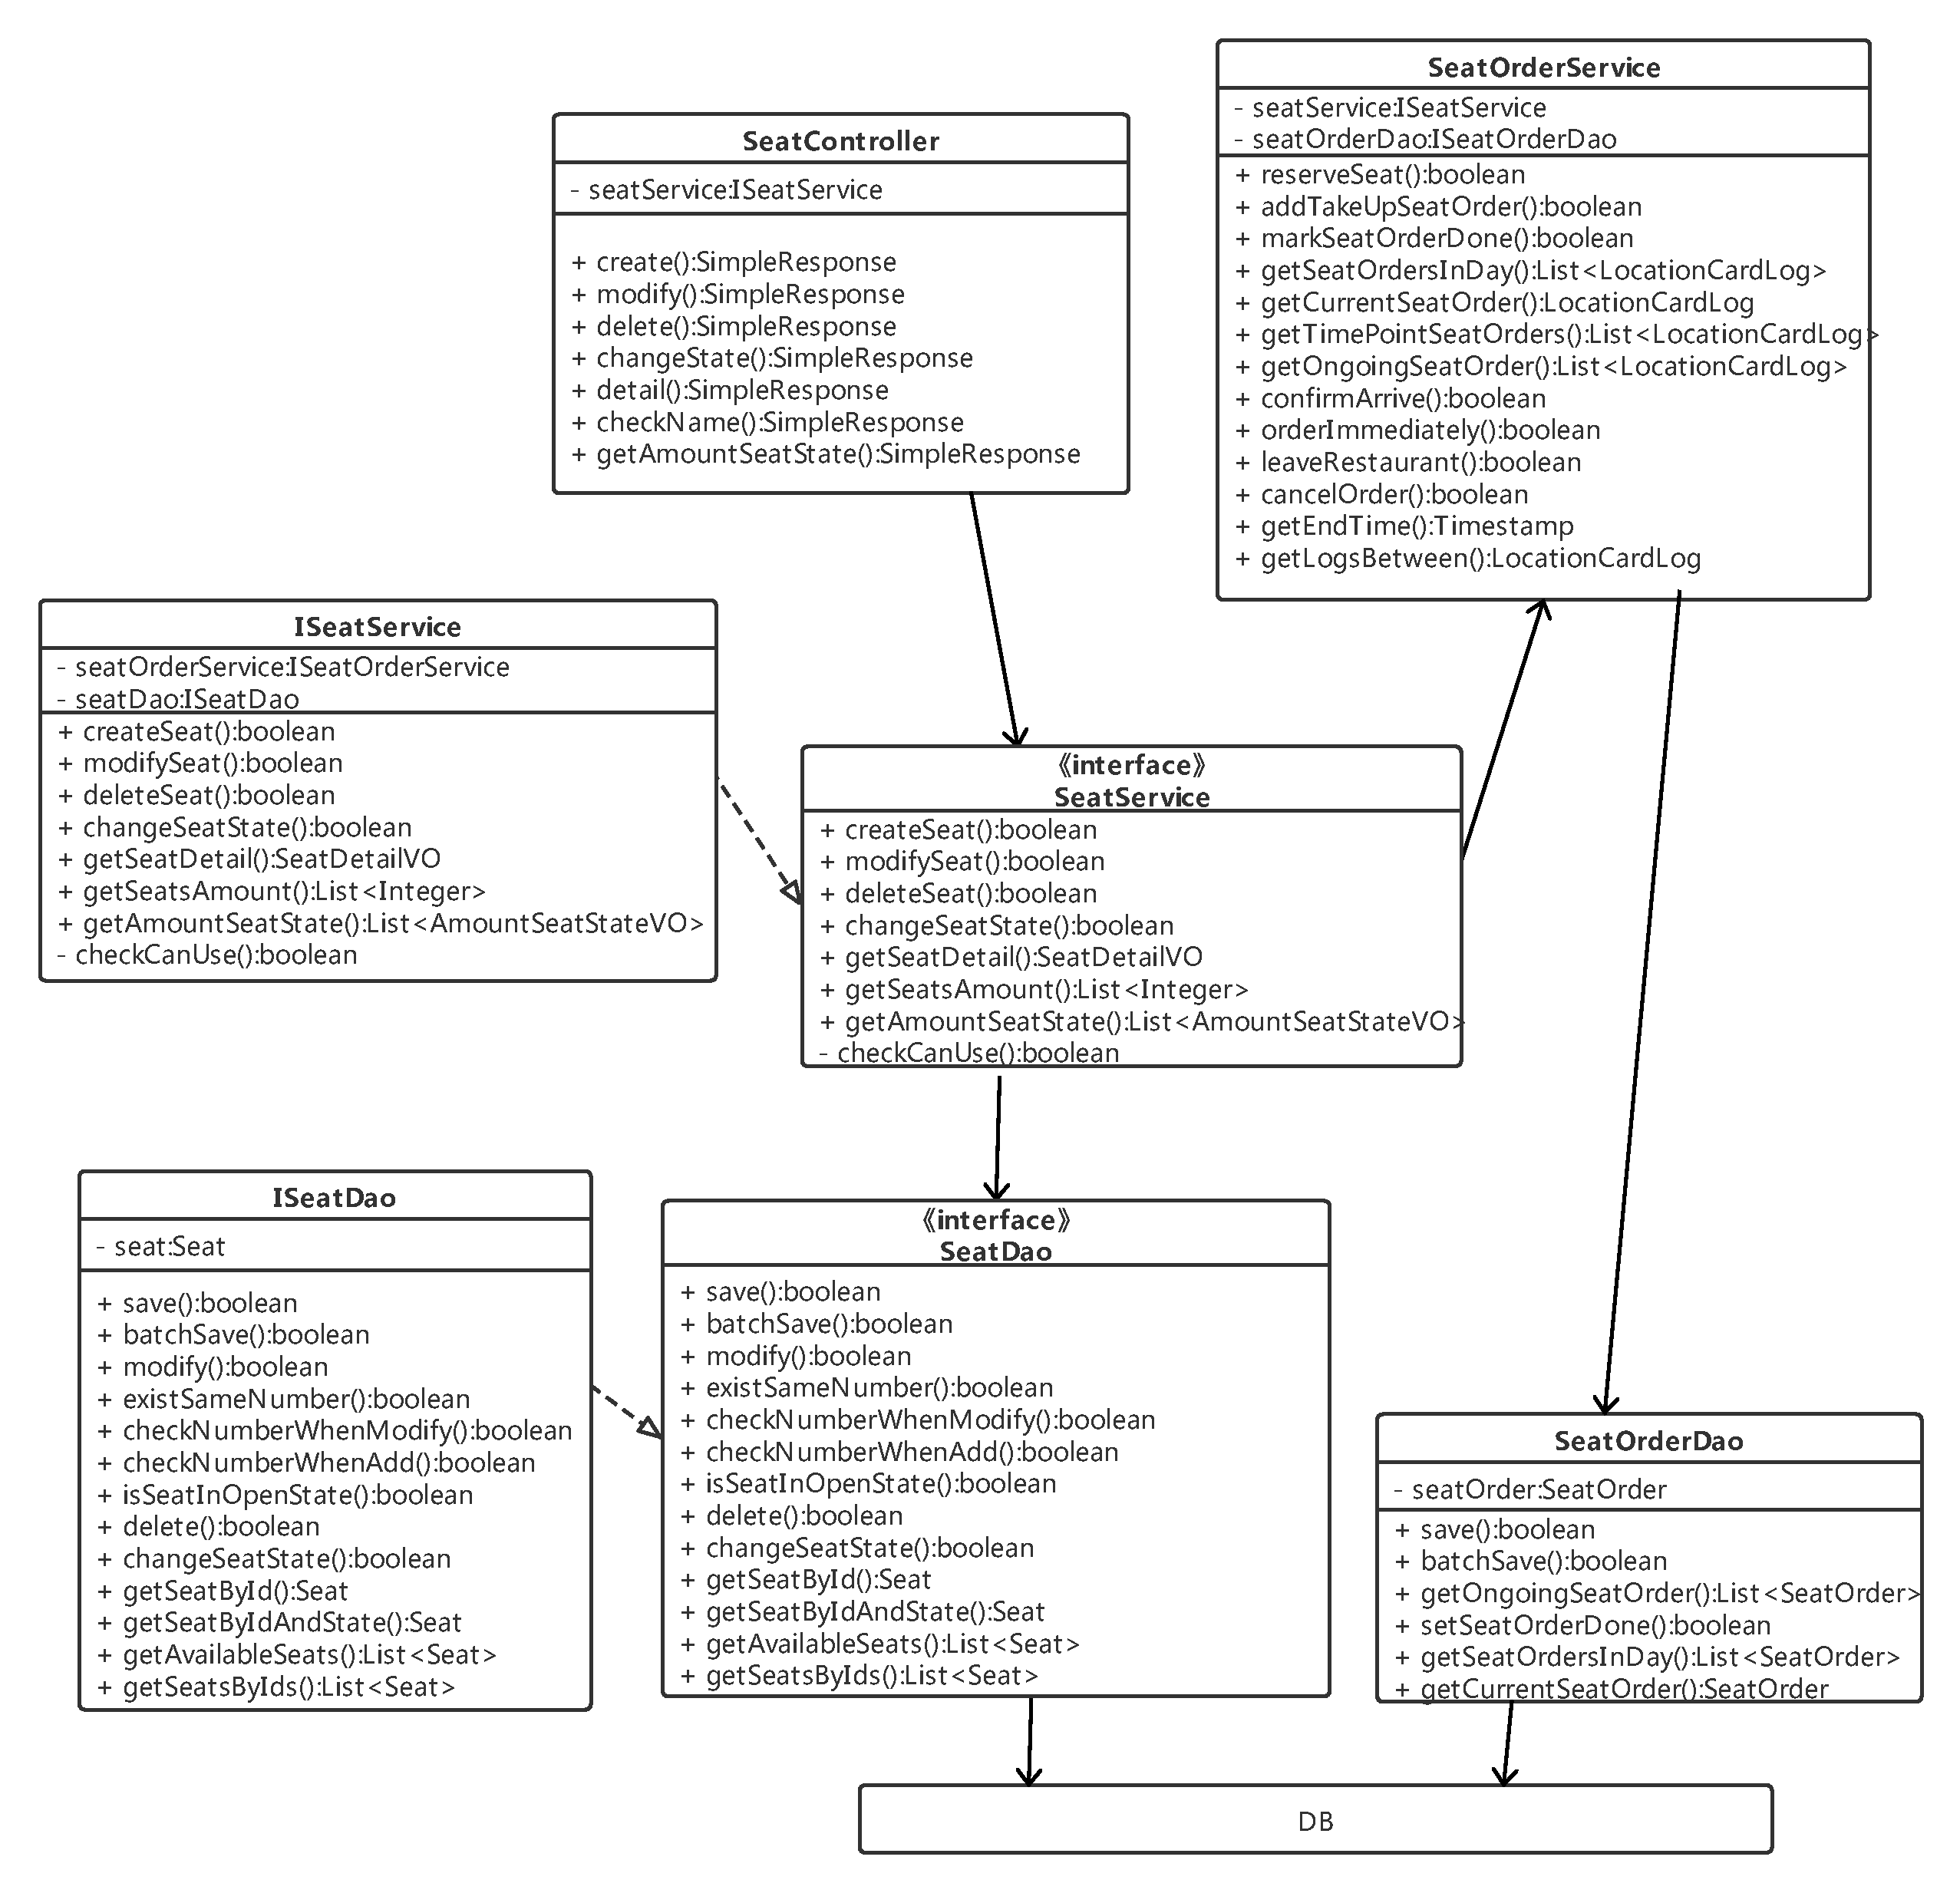
\includegraphics[width=\linewidth]{FIGs/chapter4/seat.pdf}
    \caption{座位管理模块类图}\label{fig_seat}
\end{figure}

如图~\ref{fig_seat}所示是座位管理模块的类图,这里涉及的几个类分别是:
SeatController类是座位控制接口,可以查看三种视图的座位列表,创建、修改、删除座位,修改座位状态,查看座位详情,检查座位名称是否重复,获取可用座位数量等~\cite{qjh2019}。
SeatService类是座位管理服务接口,主要提供增删改查座位、获取座位数量、获取座位详情、获取可用座位数量、更改座位状态等服务,其中ISeatService是它的实现类。
SeatOrderService类是座位订单管理服务接口,主要提供预订座位、增加占用座位订单、标记座位订单完成、获取某座位当前记录、获取时间点座位列表、获取座位使用记录、确认到店、获取时间段内座位日志等服务。
SeatDao主要用于提供座位增删改查、检索名称是否有重复、座位是否为开放状态等基本操作,其中ISeatDao是它的实现类。
SeatOrderDao主要提供座位订单的相关基本操作,比如标记座位订单完成、获取正在进行的座位订单、获取当天的座位被调用详情、获取当前时间点座位记录等,其中ISeatOrderDao是它的实现类。\\

\subsection{座位管理模块实现}
\begin{figure}[htbp!]
    \centering
    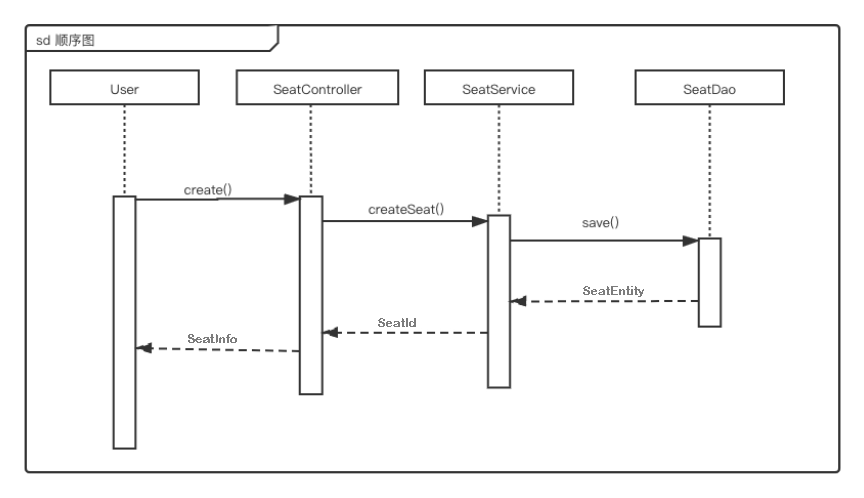
\includegraphics[width=\linewidth]{FIGs/chapter4/seat_time.pdf}
    \caption{创建座位的时序图}\label{fig_seat_time}
\end{figure}

如图~\ref{fig_seat_time}所示是SeatController类create方法的执行时序图,用户点击创建座位,填写完内容点击创建会调用SeatService类中的createSeat方法,进而调用SeatDao的save将座位内容保存到数据库中~\cite{jzh2019}。座位创建完成后会返回success信息给前端,再重新调用获取座位列表的接口来更新座位列表的界面,显示最新内容。

\begin{figure}[htbp!]
    \centering
    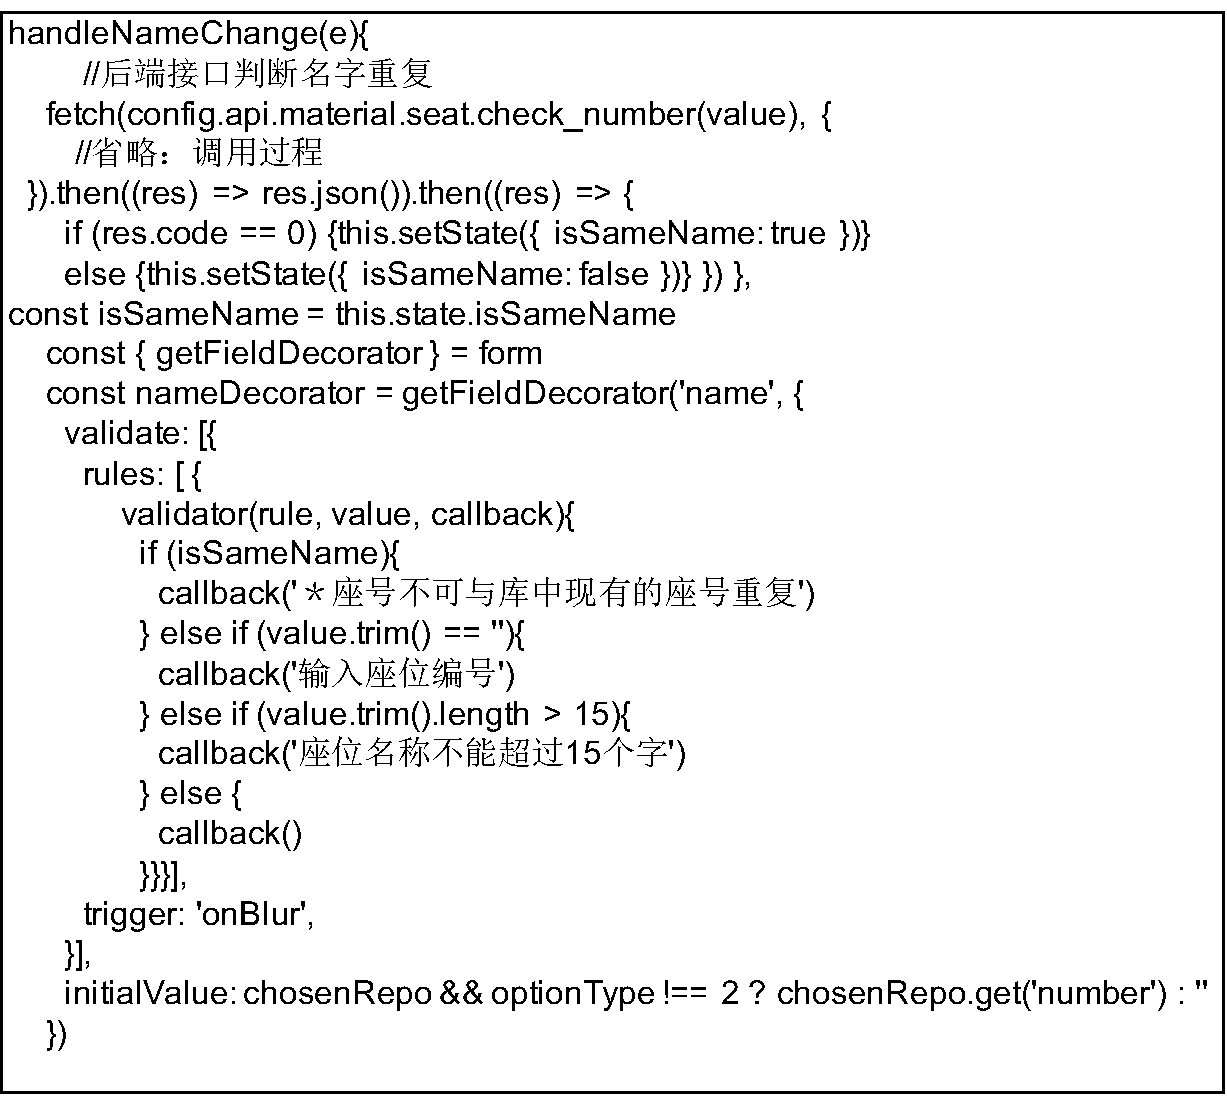
\includegraphics[width=5in]{FIGs/chapter4/8.pdf}
    \caption{前端AddSeatModal类渲染界面部分代码}\label{fig_seat_8}
\end{figure}

\begin{figure}[htbp!]
    \centering
    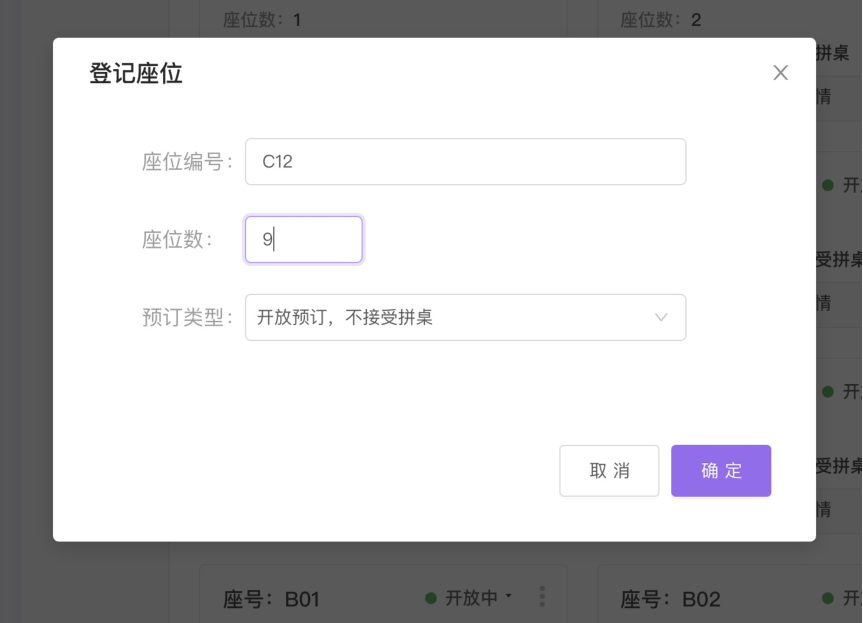
\includegraphics[width=4in]{FIGs/chapter4/seat_add.pdf}
    \caption{登记座位}\label{fig_seat_add}
\end{figure}

如图~\ref{fig_seat_8}代码所示是创建座位时,前端对座位名称的限制,座位号必填,不可与座位库中现有的座号重复而且字数限制在15字符以内。代码自定义编写了一个校验座位名称输入的规则,需要调用后端接口判断座位名是否与数据库存储内容重复。

如图~\ref{fig_seat_add}所示为登记座位页面,用户需要输入座位编号、座位数以及预订类型,点击确定完成座位的登记。

座位登记完,座位库会进行刷新显示最新的座位列表,商家可以点击相应座位查看座位详情。顾客在座位可用情况下,可以用手机扫描座位二维码进入点餐页面。

\begin{figure}[htbp!]
    \centering
    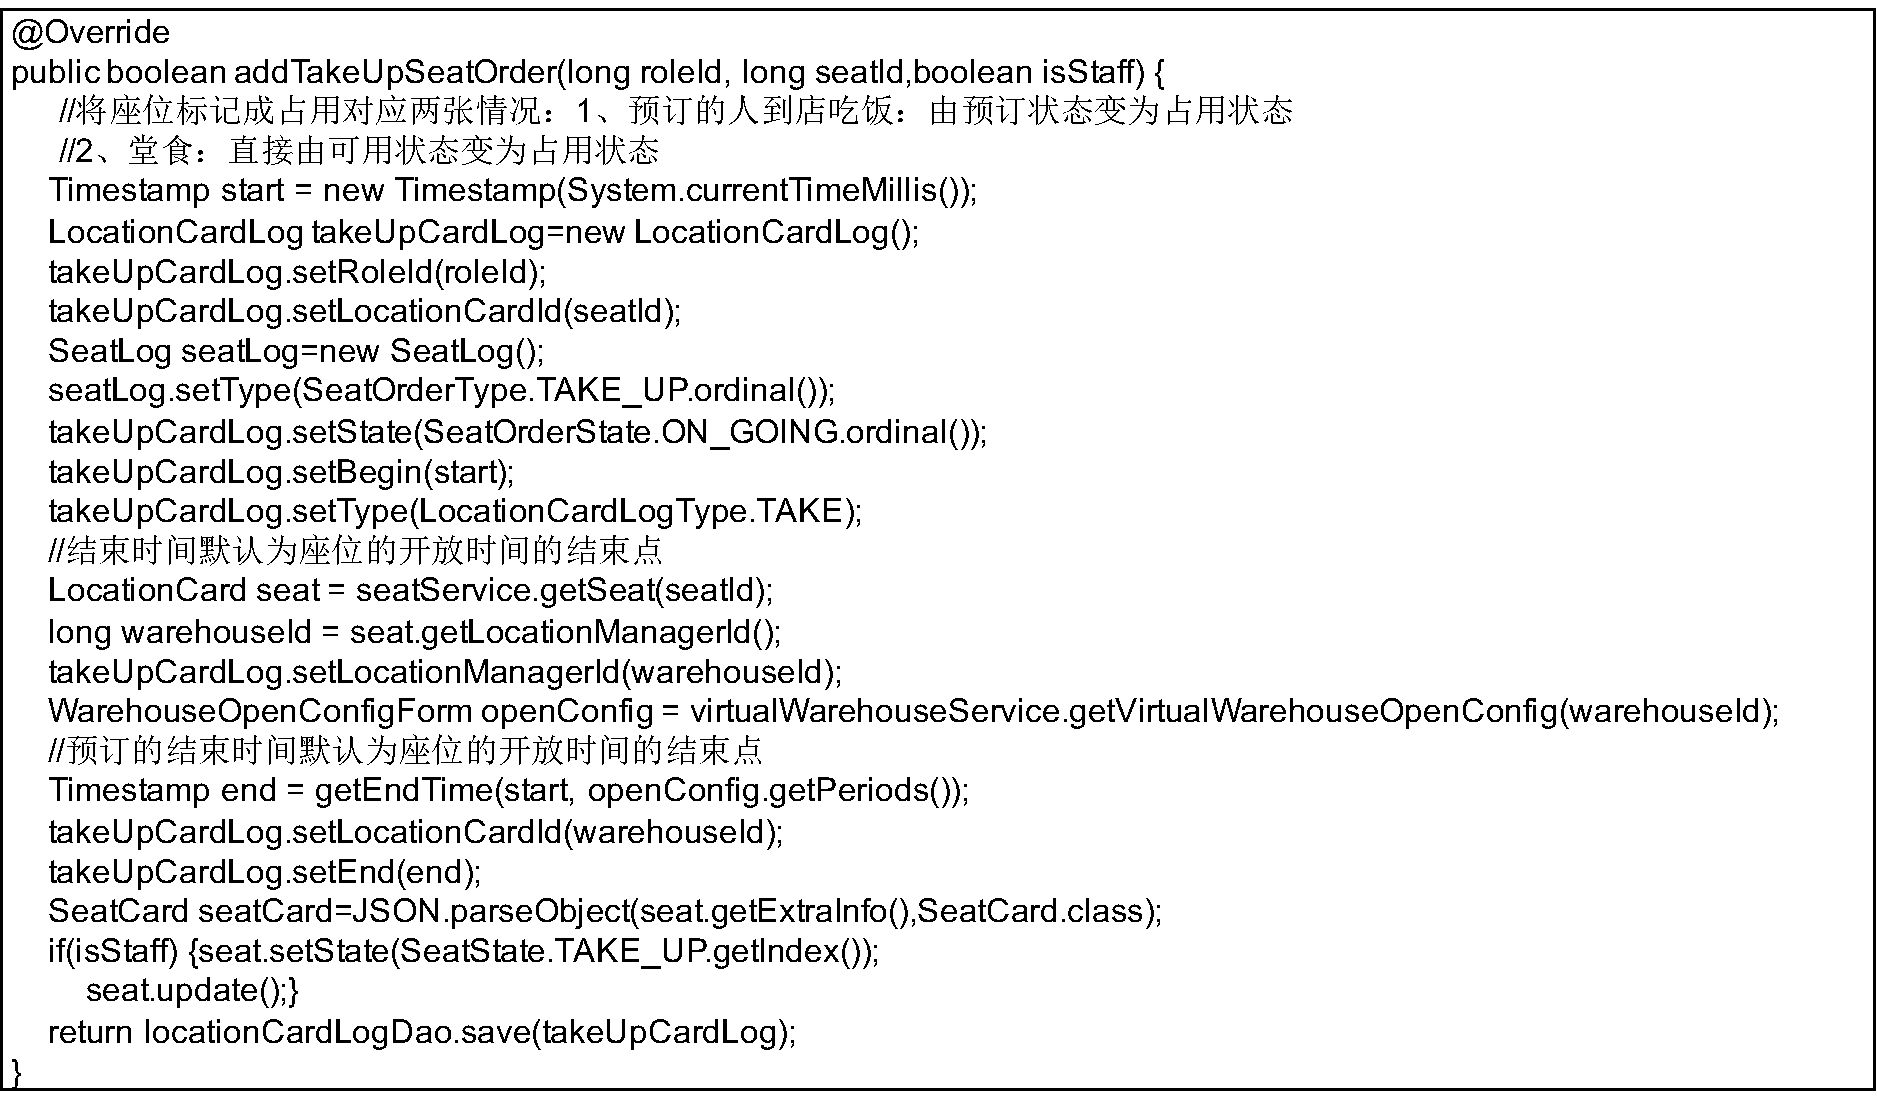
\includegraphics[width=\linewidth]{FIGs/chapter4/9.pdf}
    \caption{SeatOrderService类addTakeUpSeatOrder方法代码}\label{fig_seat_9}
\end{figure}

如图~\ref{fig_seat_9}所示是SeatOrderService类中addTakeUpSeatOrder方法的实现代码,该方法在顾客用餐时,将座位标记成占用状态并记录结束时间。座位变为占用状态有两种需要考虑的情况,一种是顾客到店用餐,座位直接变成占用状态;一种是顾客预约点单,在预约的相应时间段内座位会显示为占用状态。预约点单的结束时间可以由商家设置,如果未设置,则将默认为座位开放时间的结束点。代码通过SeatLog记录该座位的日志内容,包括占用情况、占用状态、开始结束时间等内容。

\begin{figure}[htbp!]
    \centering
    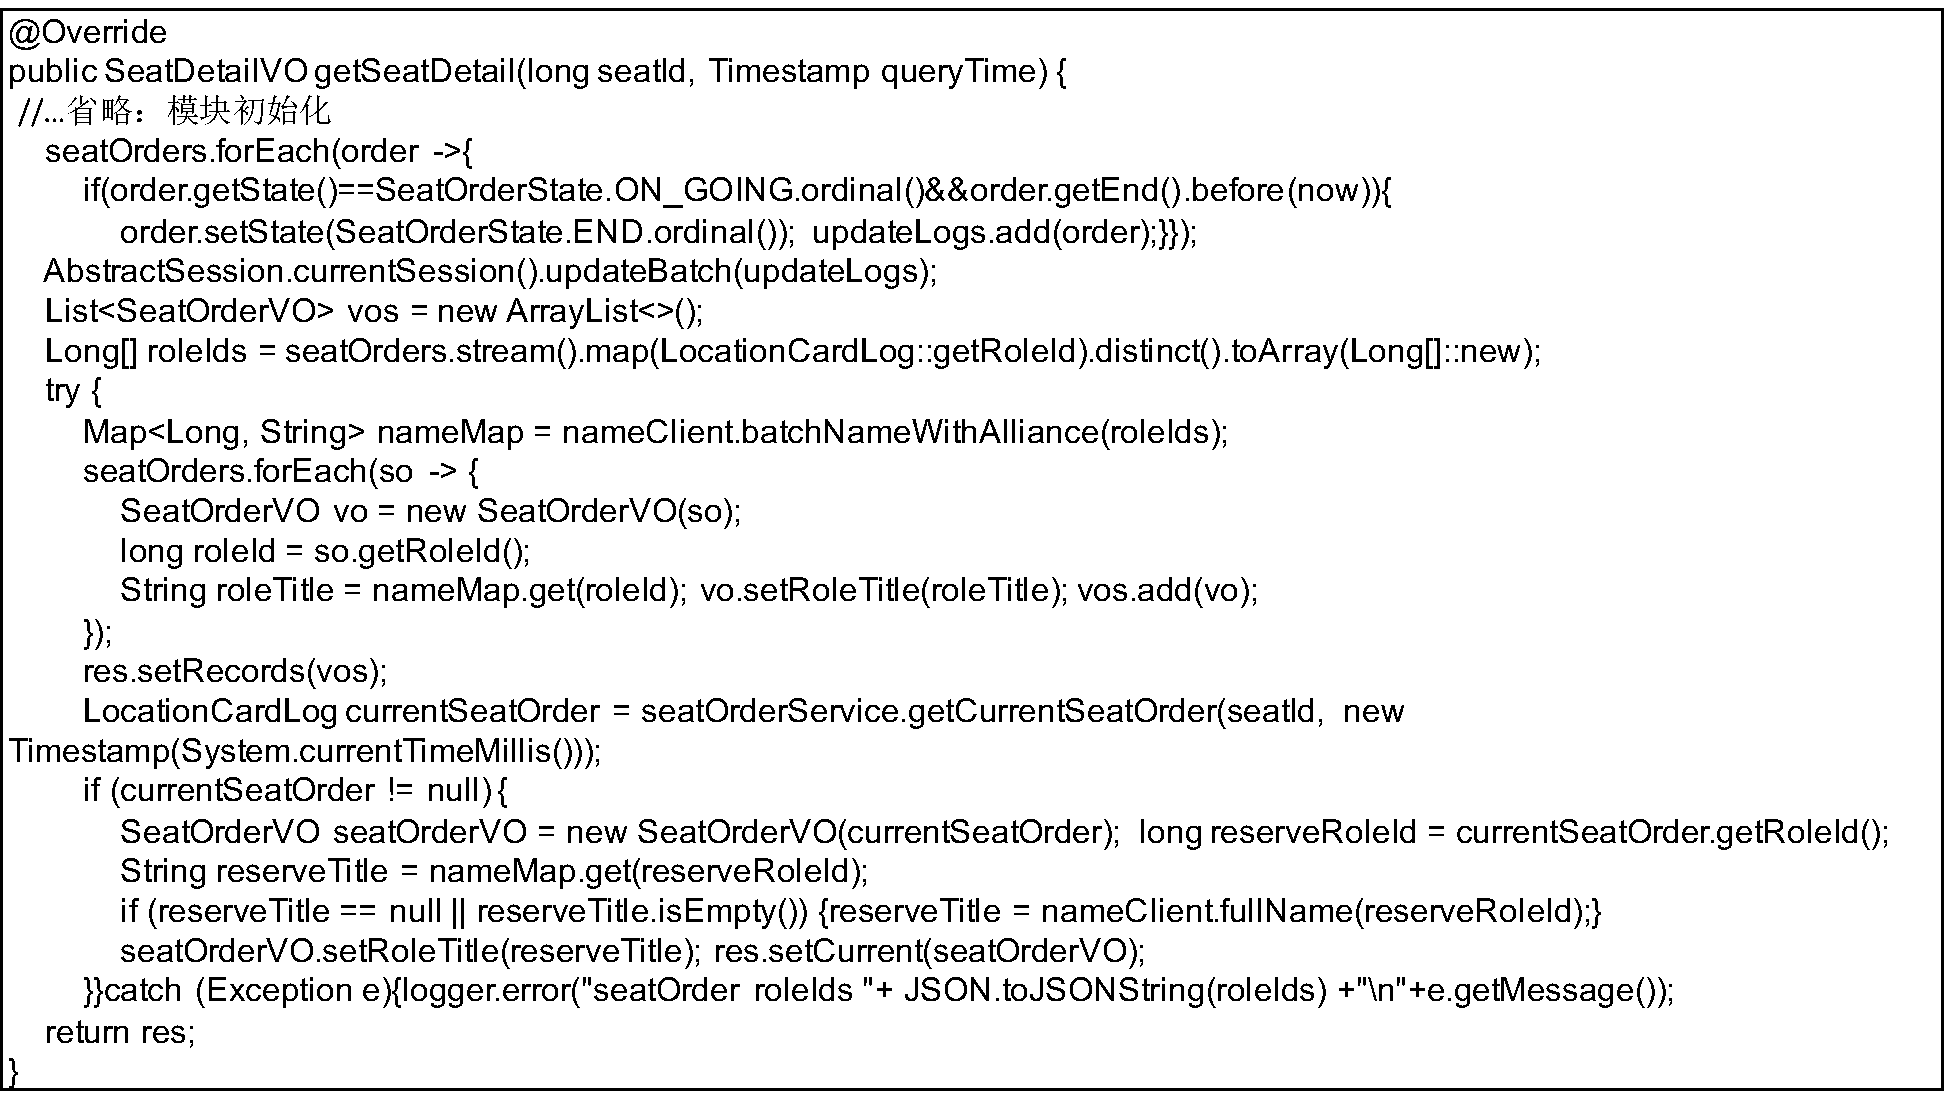
\includegraphics[width=\linewidth]{FIGs/chapter4/10.pdf}
    \caption{SeatService类中getSeatDetail方法代码}\label{fig_seat_10}
\end{figure}

\begin{figure}[htbp!]
    \centering
    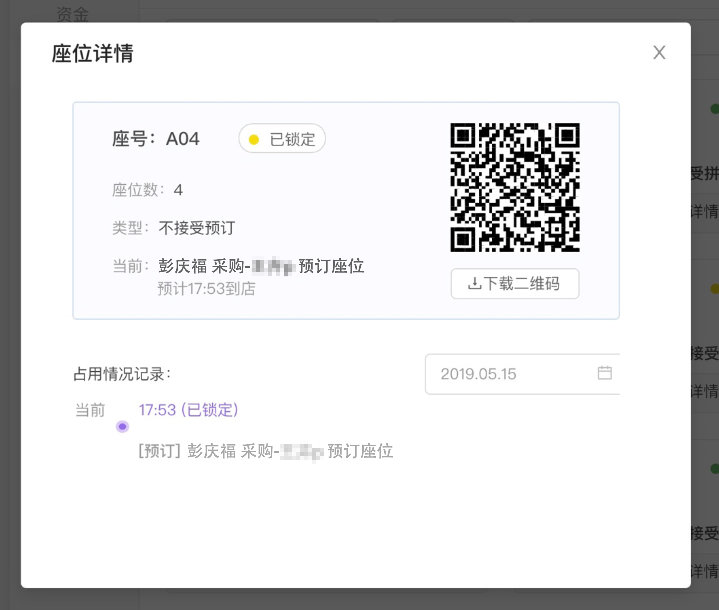
\includegraphics[width=4in]{FIGs/chapter4/seat_detail.pdf}
    \caption{座位详情}\label{fig_seat_detail}
\end{figure}

如图~\ref{fig_seat_10}所示是SeatService类中getSeatDetail方法的实现代码,该方法用于获取当天的座位详情,除了座位基本的座位号、状态、二维码、类型、当前使用情况等内容,还包括历史记录、获取座位在某时间段内的使用情况(包括预订、到店等被占用场景)~\cite{dyh}。

系统获取座位详情时,需要获取座位当前的状态,根据传入的时间获取历史占用记录。座位的二维码对应相应的座号,商家可以下载二维码将其贴到餐厅的相应位置上,以供顾客扫码点单使用。当二维码有更新或者该座位停用时,商家只需要重新下载并更换二维码即可。

如图~\ref{fig_seat_detail}所示即为某一特定座位详情,可以看到完整的座位信息,点击下载座位二维码。还可以查看座位的当前操作、根据时间筛选查看不同日期的座位占用情况记录等。

\begin{figure}[htbp!]
    \centering
    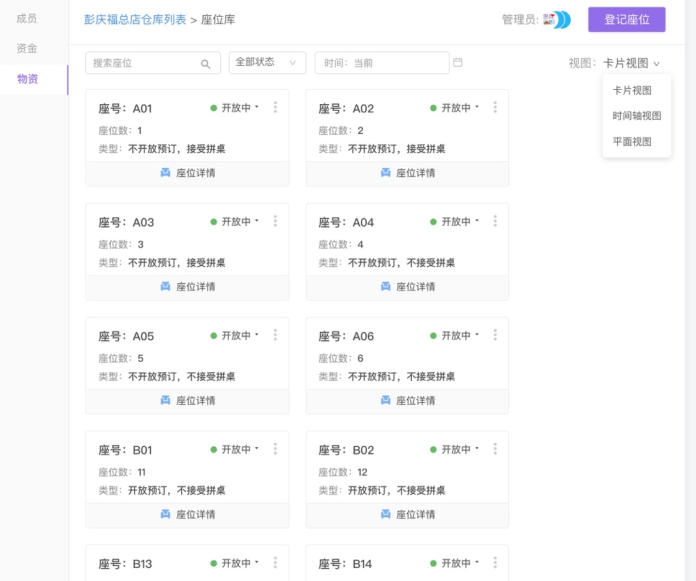
\includegraphics[width=5in]{FIGs/chapter4/seat_list.pdf}
    \caption{座位卡片视图列表}\label{fig_seat_list}
\end{figure}

如图~\ref{fig_seat_list}所示为座位库的卡片视图,可以查看餐厅内所有座位,根据座号、状态、时间筛选座位,查看相应的座位卡片内容。有操作权限的商家可以登记座位、更改座位状态、查看座位详情,还可以选择时间轴视图、平面视图进行相应信息查看和操作。

\begin{figure}[htbp!]
    \centering
    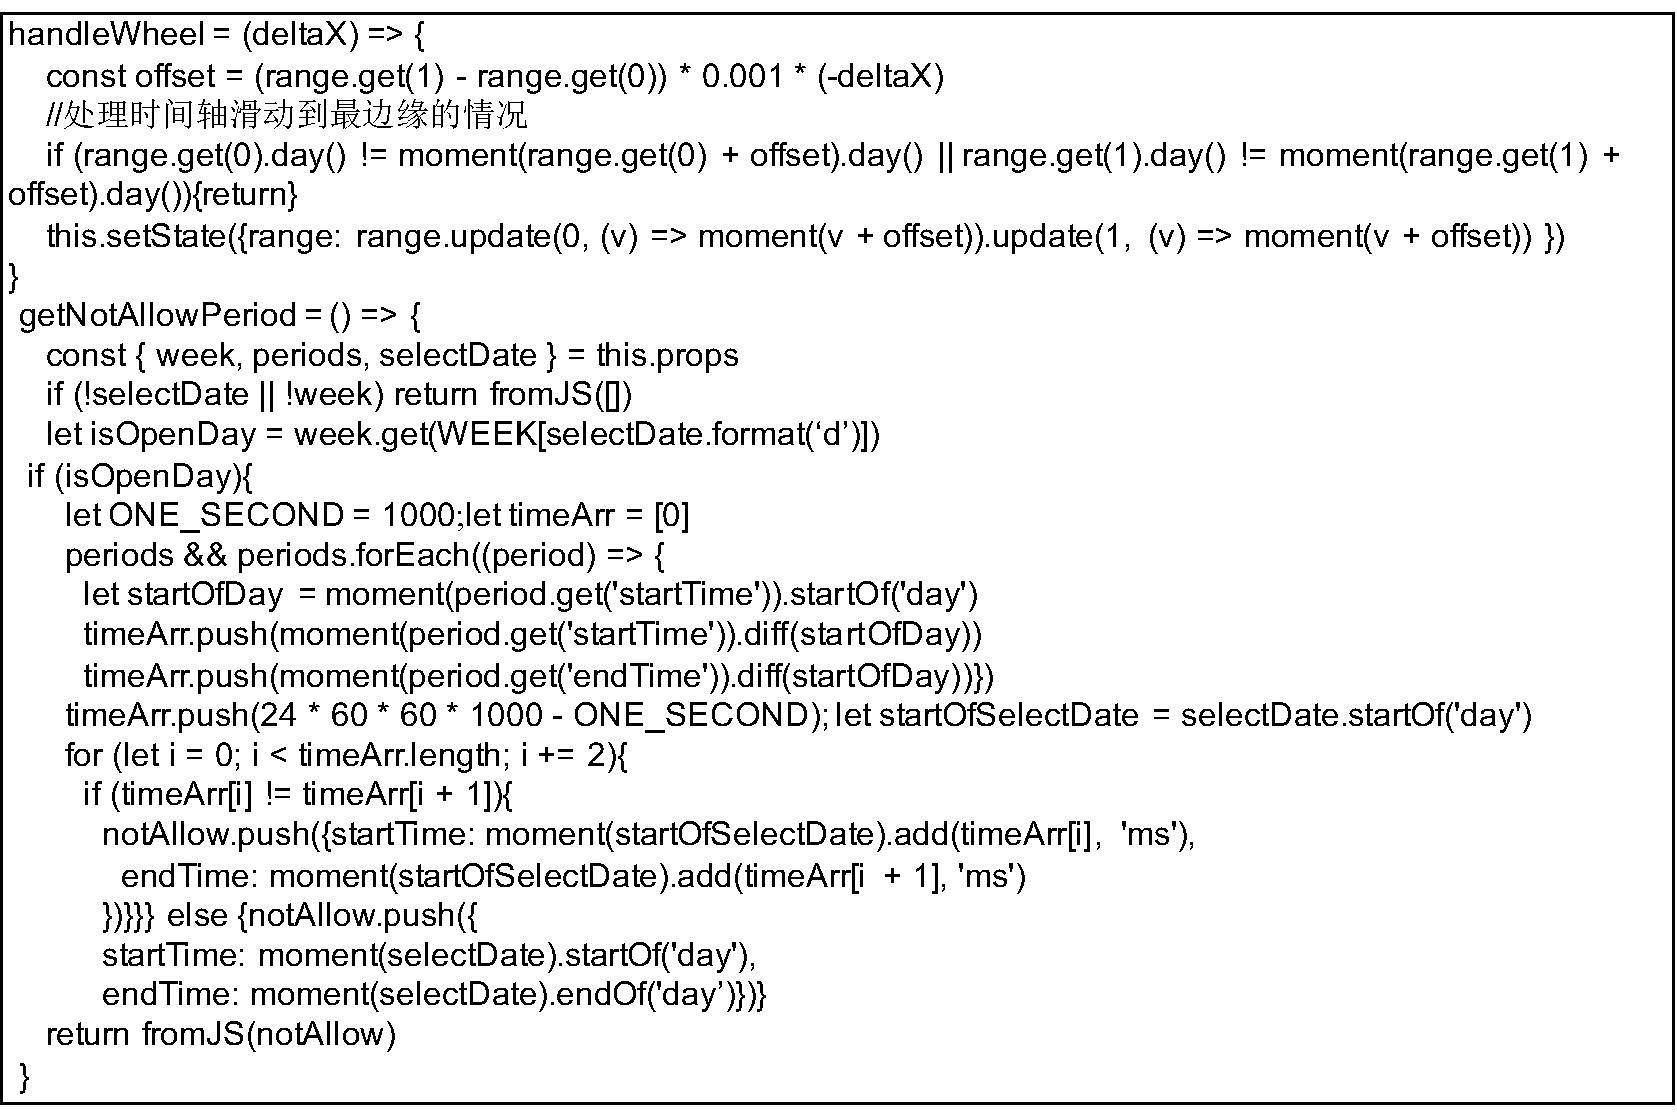
\includegraphics[width=5in]{FIGs/chapter4/11.pdf}
    \caption{实现时间轴视图SeatTimelineContainer类代码片段}\label{fig_seat_11}
\end{figure}

\begin{figure}[htbp!]
    \centering
    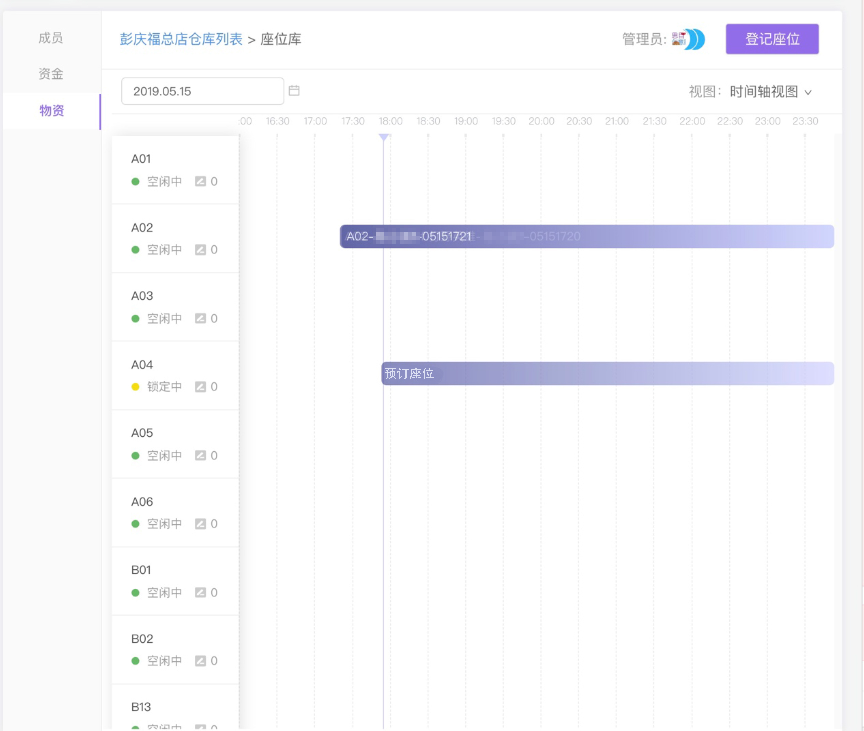
\includegraphics[width=5in]{FIGs/chapter4/seat_time_view.pdf}
    \caption{座位库时间轴视图}\label{fig_seat_time_view}
\end{figure}

座位库除了卡片视图,还可以切换成时间轴视图,查看特定日期内座位的使用情况。如图~\ref{fig_seat_11}所示是前端SeatTimelineContainer类中处理鼠标划到视图边缘情况的方法以及获取不开放时间段内容的代码片段,该类除了显示座位信息(包括座位号、状态、可用人数等),还显示座位在某一日期内24小时的占用情况(包括预订、占用中等),根据餐厅的开放时间以及各个座位的历史状态进行渲染。

如图~\ref{fig_seat_time_view}所示为座位库的时间轴视图界面,商家除了可以在该界面登记座位外,还可以根据不同日期来筛选查看座位使用情况的历史记录。

座位库除了以上两种视图外,还可以切换成平面视图,该视图结合了React封装的高德地图组件React-AMap,可以使用高德地图,也可以导入本地图片做地图,对地图上位置画圈或者打点来关联座位。
将相关联的座位卡片拖到地图上即可进行位置打点,也可以在地图上画一个完整的多边形区域,将卡片拖拽进区域内与位置相关联。

平面视图主要为了将餐厅与线下实际位置绑定,顾客可以在地图上直观看到区域划分。防止虚假定位欺骗消费者,也方便商家将餐厅内部的座位布局上传到系统内,与座位库的座位进行关联绑定,更方便直观的管理餐厅普通座位、拼桌座位、包厢等。

\begin{figure}[htbp!]
    \centering
    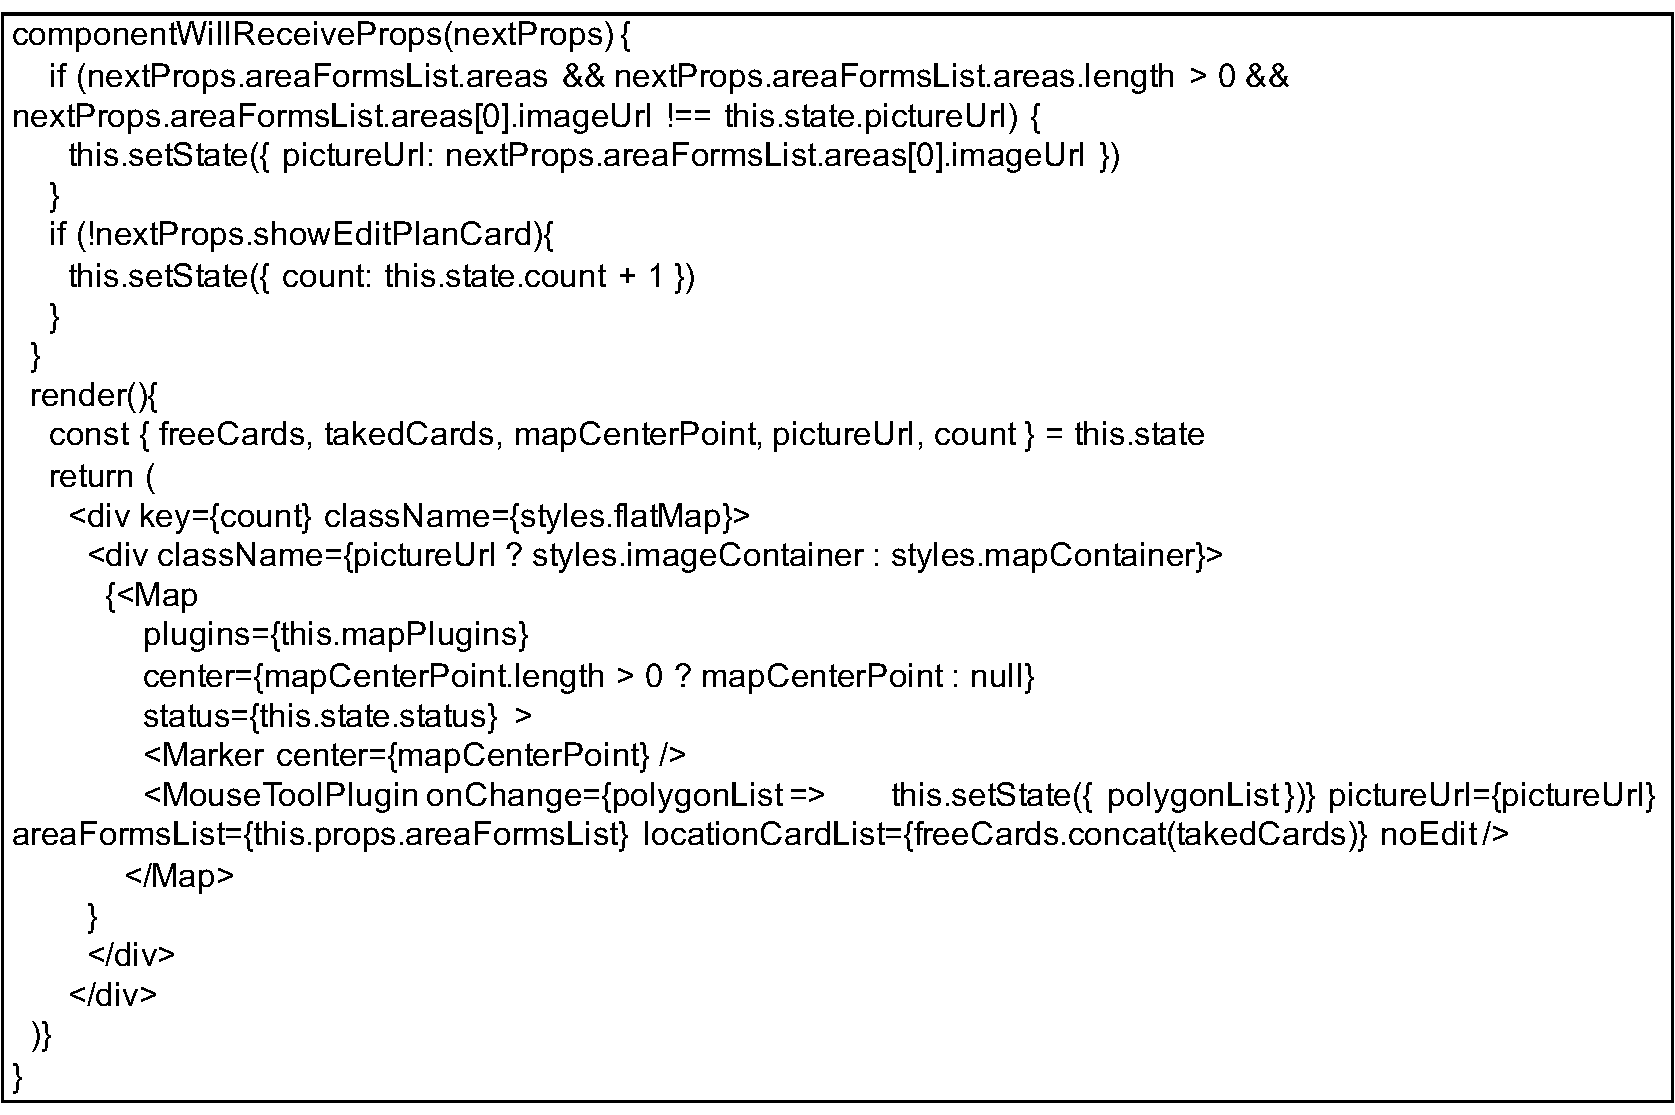
\includegraphics[width=5in]{FIGs/chapter4/12.pdf}
    \caption{实现平面视图FlatViewContainer类代码片段}\label{fig_seat_12}
\end{figure}

如图~\ref{fig_seat_12}所示为前端FlatViewContainer类部分代码,引入了React封装的高德地图组件的类库React-AMap中Map、Marker组件,自定义编写了组件类MouseToolPlugin实现地图上的自定义操作,地图更换为本地导入的图片时,该类会判断并刷新界面,将之前地图上存在的点、多边形区域和相关联的座位卡片信息清除~\cite{lzt2015}。

如图~\ref{fig_seat_13}所示,是前端类MouseToolPlugin中绘制包括地图、座位卡片、多边形以及各个坐标点的方法handleDrawAll。该方法从后端获取历史数据并渲染到地图中(包括多边形、位置点的构造),实现了将座位卡片拖到指定区域的操作,地图可以随意放大或缩小,画出的多边形区域也会随之改变。

\begin{figure}[htbp!]
    \centering
    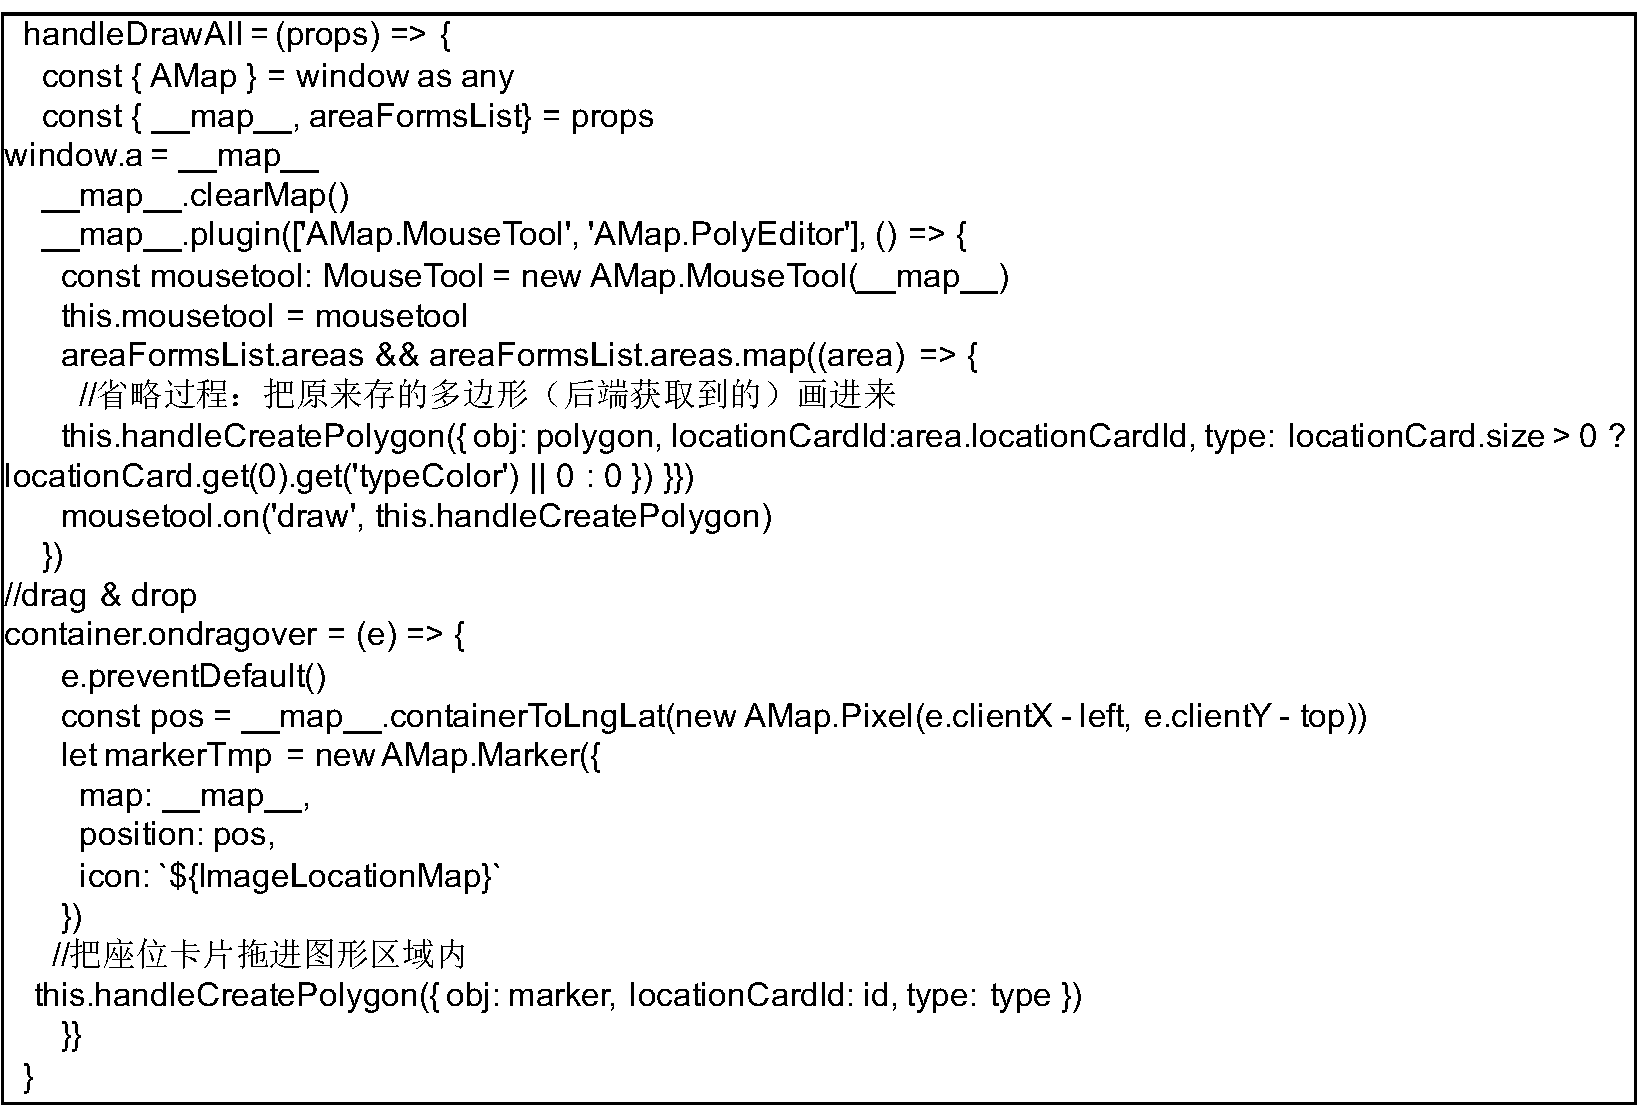
\includegraphics[width=5in]{FIGs/chapter4/13.pdf}
    \caption{MouseToolPlugin类handleDrawAll方法代码}\label{fig_seat_13}
\end{figure}

需要判断平面视图的底图是高德地图还是用户自定义上传的餐厅图片,如果是地图则直接引用React-AMap组件地图进行简单修改即可,该组件支持任意程度的放大、缩小、移动。如果是用户上传的自定义图片,需要进行边界校验,当图片显示为100\%的时候,禁止缩小与移动,保证图片填充满整个地图界面,图片放大时才可以拖拽图片,当到达图片边缘时,图片不能再往边缘方向拖动。

\begin{figure}[htbp!]
    \centering
    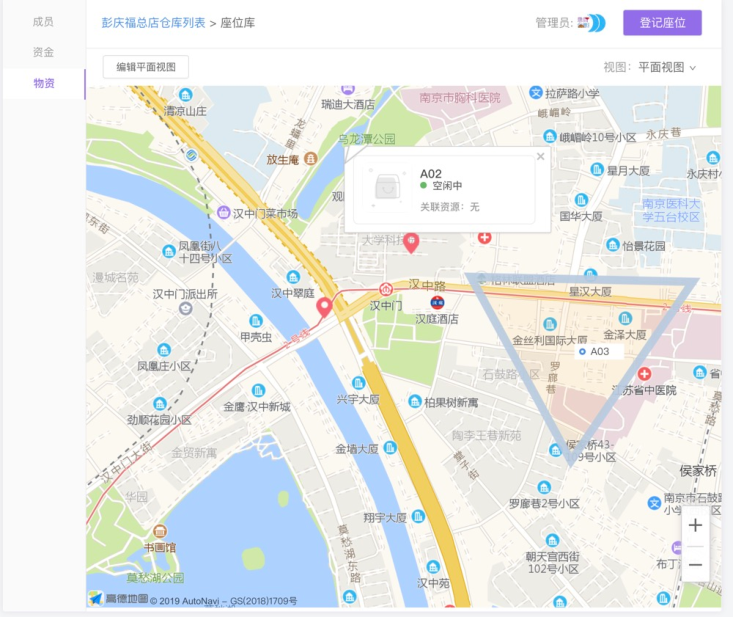
\includegraphics[width=5in]{FIGs/chapter4/seat_map.pdf}
    \caption{座位库平面视图}\label{fig_seat_map}
\end{figure}

\begin{figure}[htbp!]
    \centering
    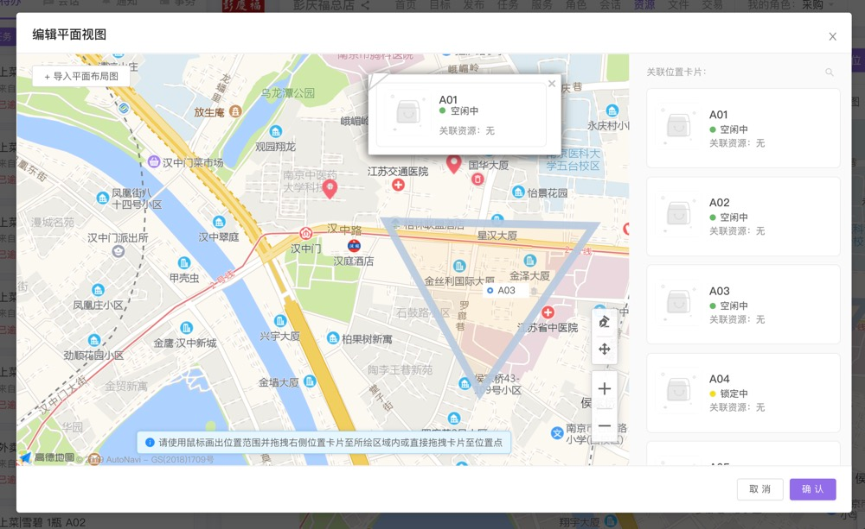
\includegraphics[width=5in]{FIGs/chapter4/seat_map_edit.pdf}
    \caption{编辑平面视图}\label{fig_seat_map_edit}
\end{figure}

如图~\ref{fig_seat_map}是座位库的平面视图,地图中的多边形区域和坐标点都有与之相关联的座位卡片。鼠标点击某个点或者某个多边形中的座位号时,即显示图中具体的座位信息内容,包括座号、状态、关联资源等内容~\cite{wzz2016}。

如图~\ref{fig_seat_map_edit}所示为编辑平面视图界面,默认地图会显示当前位置,用户可以点击导入平面布局图,可以上传自定义图片。用户可以将右边的座位卡片拖拽到左边地图中形成一个坐标点,点击即可查看相关联的座位信息;也可以先在左边地图中用钢笔工具画出一个闭环的多边形区域,再将座位卡片拖拽进多边形实现位置与卡片相关联。\\

\section{出品发布模块}
\begin{figure}[htbp!]
    \centering
    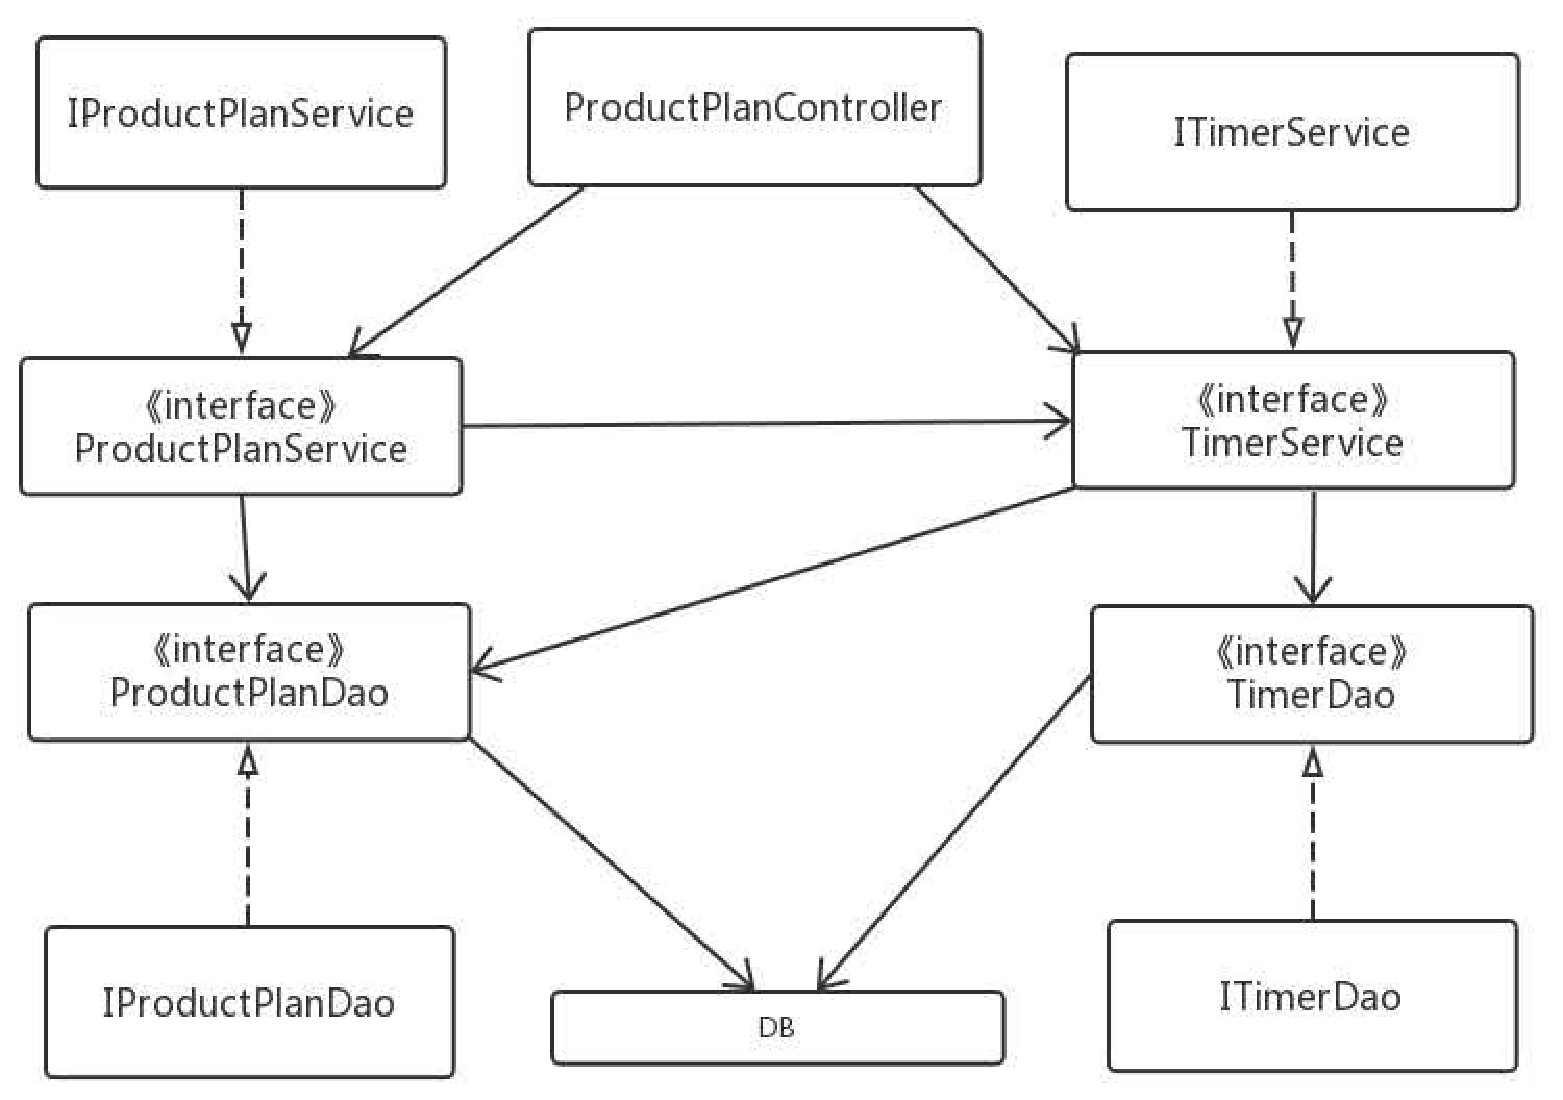
\includegraphics[width=\linewidth]{FIGs/chapter4/dish.pdf}
    \caption{出品发布模块类图}\label{fig_dish}
\end{figure}

\subsection{出品发布模块介绍}
出品发布模块主要负责每日出品计划、菜品计划、管理餐厅营业时间等,对外提供商家营业信息、出品计划、菜品信息等接口。\\

\subsection{出品发布模块详细设计}

如图~\ref{fig_dish}所示是出品发布模块的类图,这里涉及的几个类分别是:ProductPlanController类是出品发布控制接口,可以创建、修改、删除出品发布,保存草稿,获取菜单,获取开放时间,增删改出品发布时间段等~\cite{abf}。

ProductPlanService类是出品发布服务接口,主要提供增删改查出品计划、获取出品发布详情、上架出品发布、根据出品发布获取菜单、获取当前上架的发布ID等服务,其中IProductPlanService是它的实现类。

TimerService类是出品时间段管理服务接口,主要提供增删改出品发布时间段、获取餐厅营业的所有时间段、获取当前时间段等服务,其中ITimerService是它的实现类。

ProductPlanDao主要通过出品发布ID或者菜单获得、更新、修改、批量删除出品计划列表等基本操作,其中IProductPlanDao是它的实现类。

TimerDao主要用于提供时间相关基本操作,比如通过ID获取时间段、删除时间段、获取当前开始或者结束出品计划的时间、批量获取时间段等,其中ITimerDao是它的实现类。\\

\subsection{出品发布模块实现}

\begin{figure}[htbp!]
    \centering
    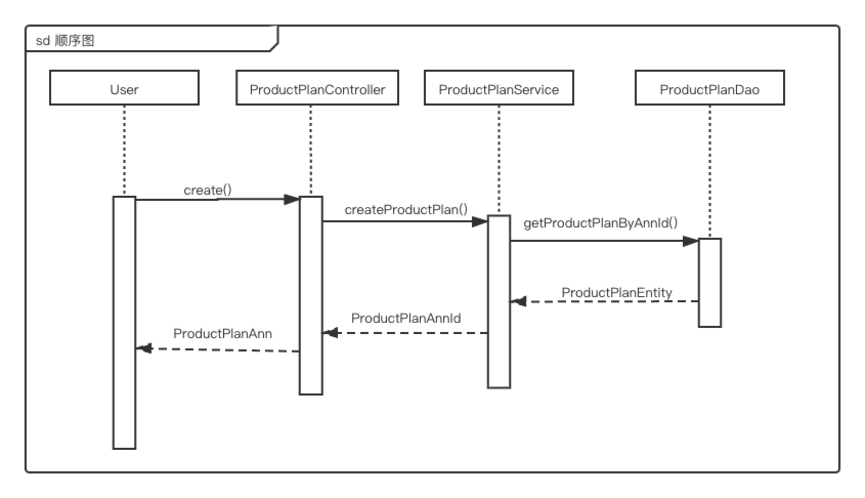
\includegraphics[width=4.5in]{FIGs/chapter4/dish_time.pdf}
    \caption{创建出品发布的时序图}\label{fig_dish_time}
\end{figure}

如图~\ref{fig_dish_time}所示是ProductPlanController类create方法的执行时序图,用户点击新建出品发布,填写完相应内容后,点击创建会调用ProductPlanService类中的createProductPlan方法,进而调用ProductPlanDao的getProductPlanByAnnId将出品发布内容保存到数据库中,并返回相应的发布ID。

如果是简单的创建出品发布,系统通过发布ID获取发布详情并返回给前端。如果是复用已有的出品发布进行创建,系统会根据复用的发布ID去获取该复用发布的出品发布详情,包括餐厅当日营业时间段、菜品列表等内容,并将其更新到创建的发布内容中,使用户不必重复创建相同内容,减少工作量。后端返回该发布ID,系统根据ID获取具体的发布详情,进行界面渲染。

\begin{figure}[htbp!]
    \centering
    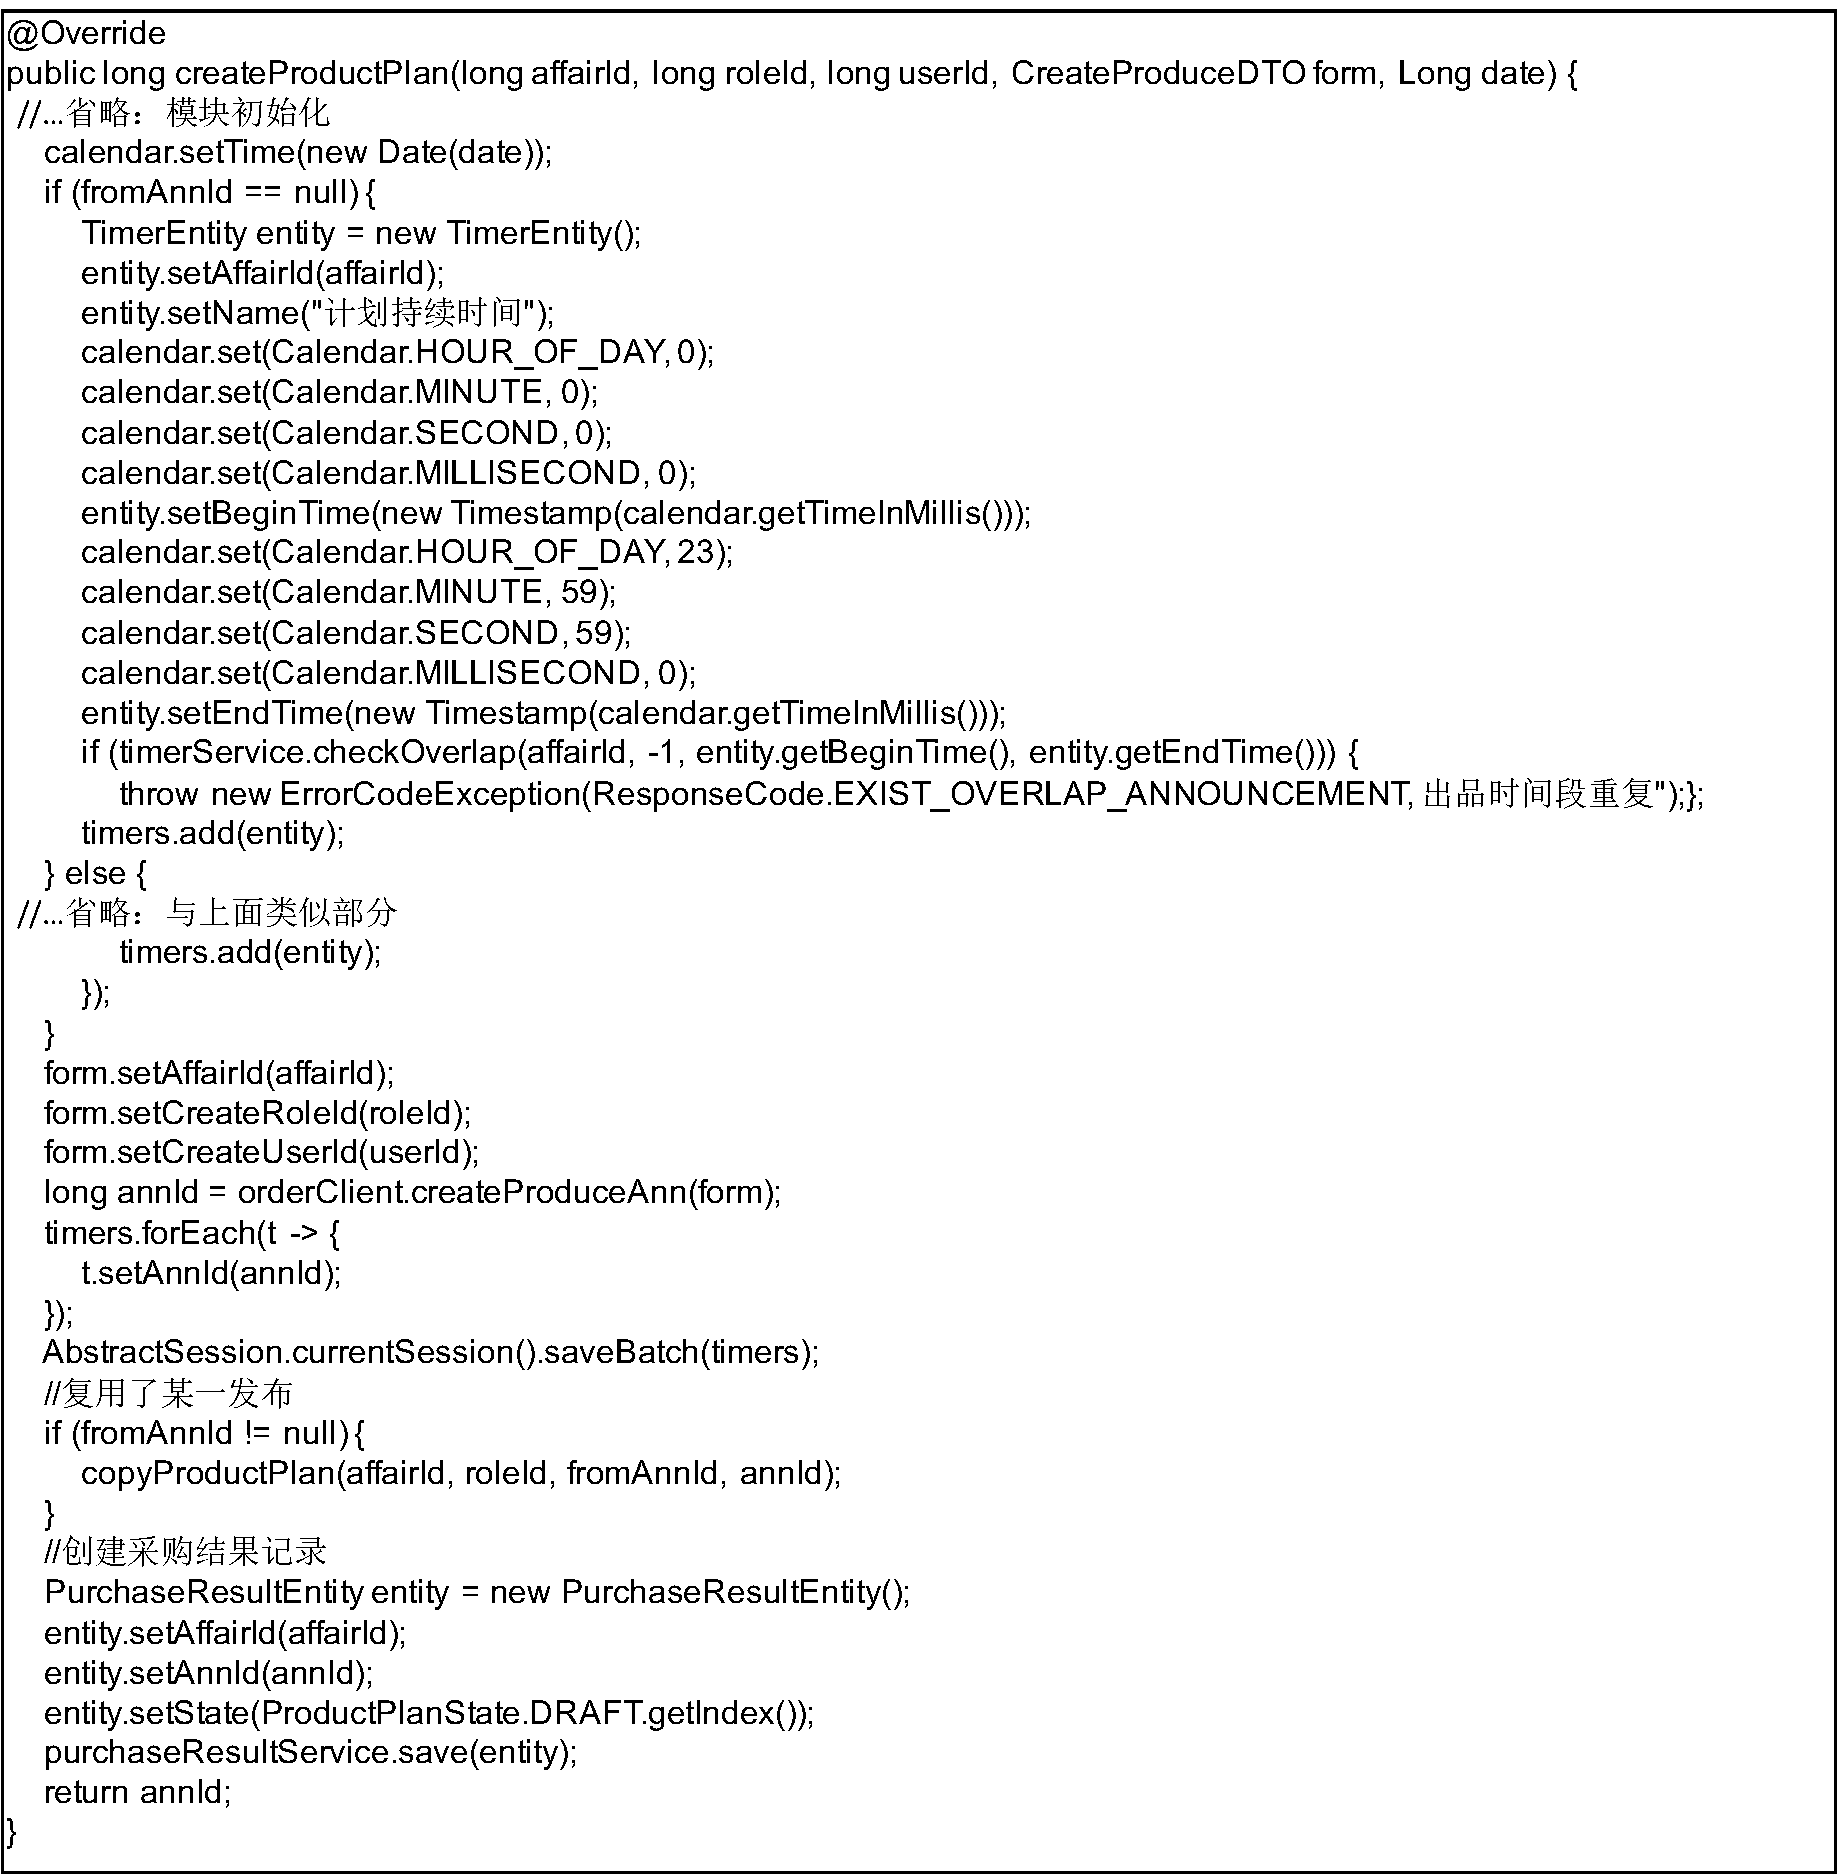
\includegraphics[width=4.5in]{FIGs/chapter4/14.pdf}
    \caption{ProductPlanService类createProductPlan方法代码}\label{fig_dish_14}
\end{figure}

如图~\ref{fig_dish_14}所示是ProductPlanService类中createProductPlan方法的实现代码,该方法用于商家创建出品发布,需要填写相应的出品计划,包括商家一天的营业时间段、是否复用之前的出品发布、选择的菜品等操作。后端会判断出品时间段是否有重复,若是则提示用户更改时间段,用户填写内容无误并成功创建出品发布后,系统返回该出品发布的发布ID~\cite{tkx2014}。

\begin{figure}[htbp!]
    \centering
    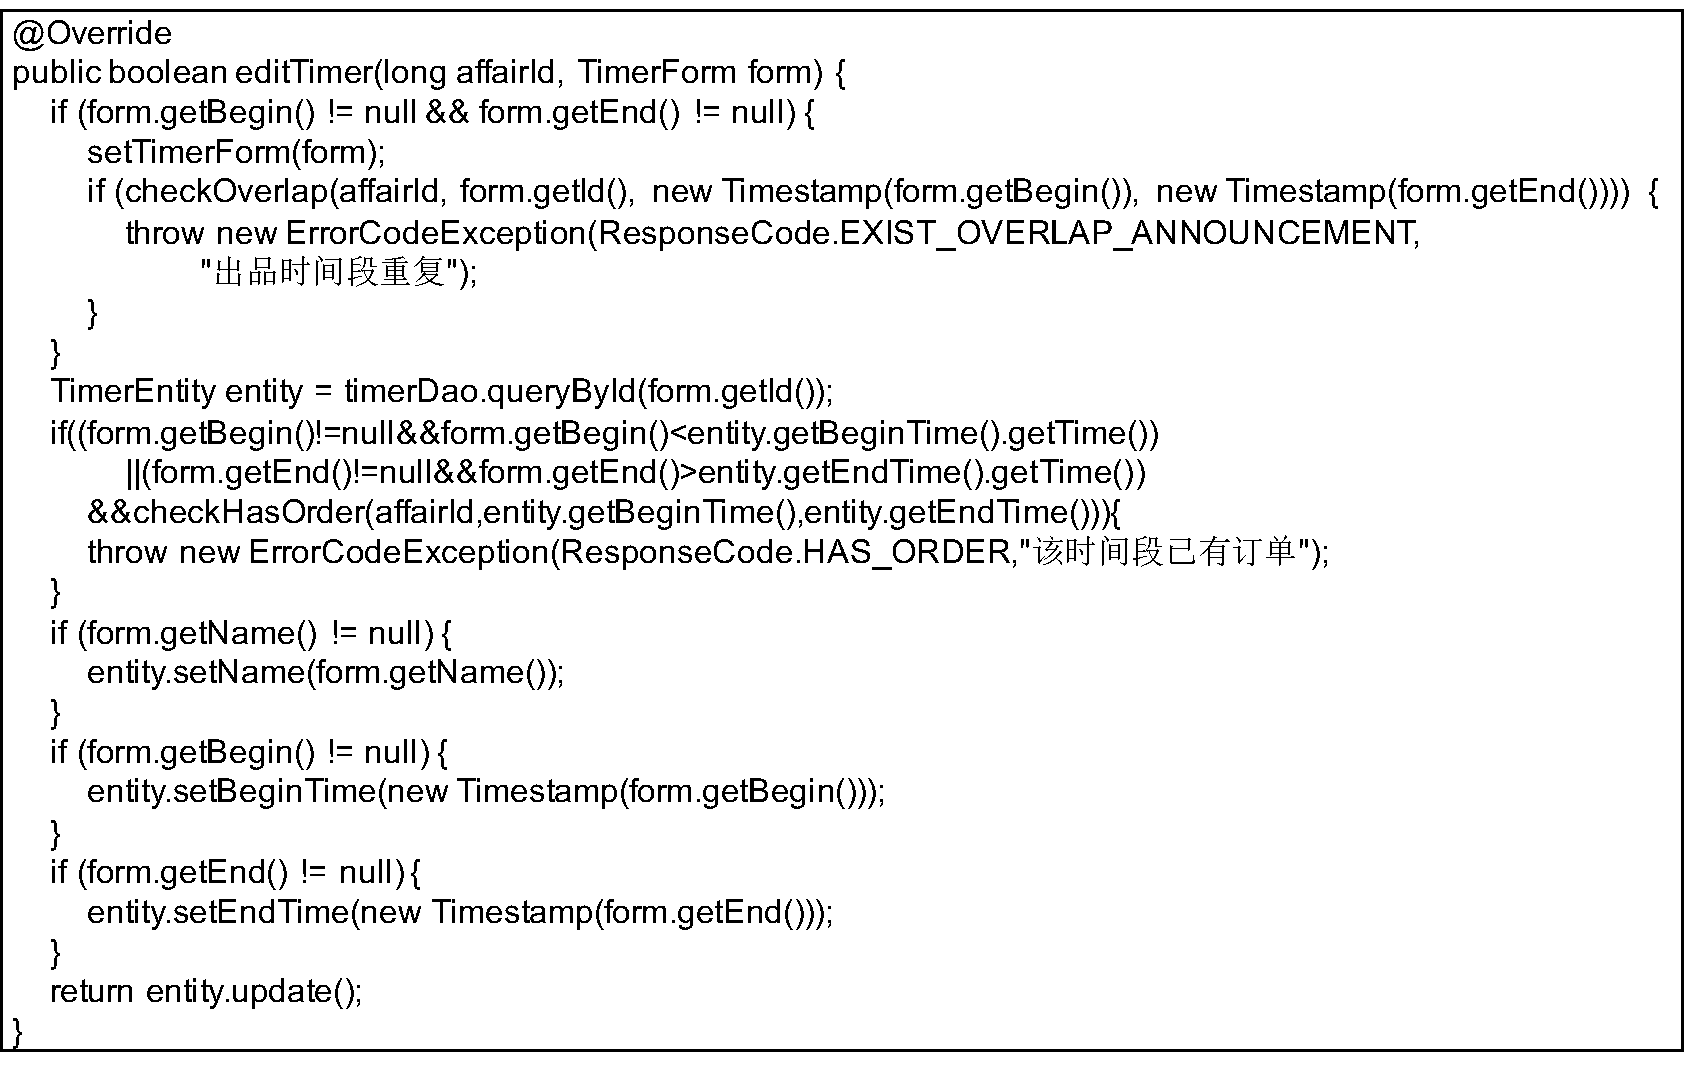
\includegraphics[width=4.5in]{FIGs/chapter4/15.pdf}
    \caption{TimerService类中editTimer方法代码}\label{fig_dish_15}
\end{figure}

\begin{figure}[htbp!]
    \centering
    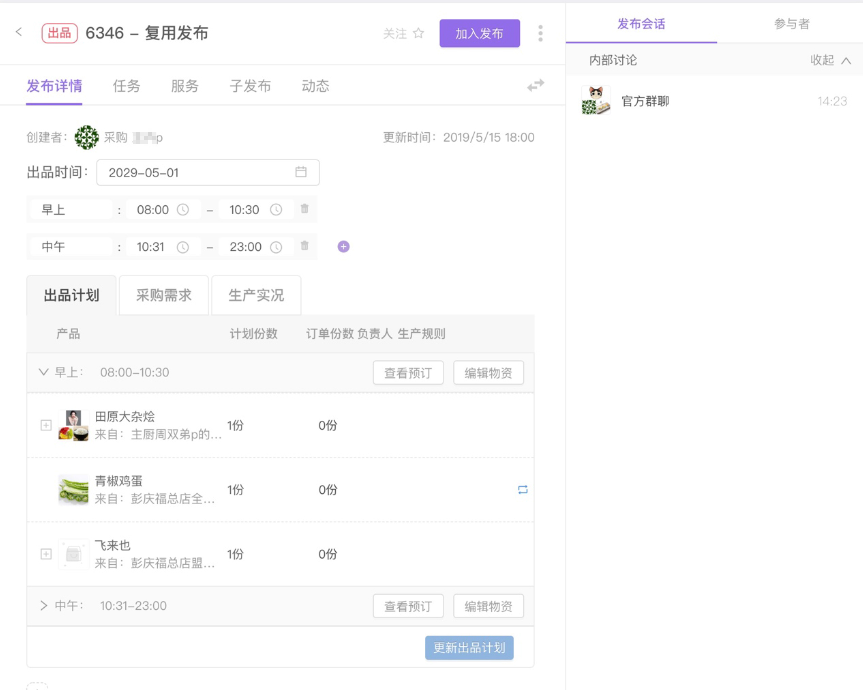
\includegraphics[width=4in]{FIGs/chapter4/dish_detail.pdf}
    \caption{出品发布详情}\label{fig_dish_detail}
\end{figure}

如图~\ref{fig_dish_15}所示是TimerService类中editTimer方法的实现代码,该方法用于修改当天出品发布的出品时间段。餐厅可能需要将营业时间分为早上营业时间、中午营业时间、晚上营业时间等多个时间段,所以修改时间段时除了需要判断结束时间不得早于开始时间,还需要判断出品时间段是否有重复,要修改的时间段是否已经有订单等。

如图~\ref{fig_dish_detail}所示为出品发布详情界面,由于该发布复用了之前的发布内容,所以创建后默认有与复用发布相同的营业时间段和出品计划菜单,商家可以修改当前发布的出品时间段、编辑时间段内的菜品种类及数量,查看采购需求、生产实况,及时上架、更新出品计划。\\

\section{本章小结}
本章首先讲解了彭庆福餐厅点单系统各个模块的依赖关系,接着分别描述了系统六个主要模块——订单发布模块、支付模块、用户管理模块、统计报表模块、座位管理模块和出品发布模块的详细设计与具体实现,通过模块类图、方法时序图、代码片段以及前端界面图来展示模块的实现细节与运行结果。